% mnras_template.tex 
%
% LaTeX template for creating an MNRAS paper
%
% v3.0 released 14 May 2015
% (version numbers match those of mnras.cls)
%
% Copyright (C) Royal Astronomical Society 2015
% Authors:
% Keith T. Smith (Royal Astronomical Society)

% Change log
%
% v3.0 May 2015
%    Renamed to match the new package name
%    Version number matches mnras.cls
%    A few minor tweaks to wording
% v1.0 September 2013
%    Beta testing only - never publicly released
%    First version: a simple (ish) template for creating an MNRAS paper

%%%%%%%%%%%%%%%%%%%%%%%%%%%%%%%%%%%%%%%%%%%%%%%%%%
% Basic setup. Most papers should leave these options alone.
\documentclass[fleqn,usenatbib,letters]{mnras}

% MNRAS is set in Times font. If you don't have this installed (most LaTeX
% installations will be fine) or prefer the old Computer Modern fonts, comment
% out the following line
\usepackage{newtxtext,newtxmath}
% Depending on your LaTeX fonts installation, you might get better results with one of these:
%\usepackage{mathptmx}
%\usepackage{txfonts}

% Use vector fonts, so it zooms properly in on-screen viewing software
% Don't change these lines unless you know what you are doing
\usepackage[T1]{fontenc}

% Allow "Thomas van Noord" and "Simon de Laguarde" and alike to be sorted by "N" and "L" etc. in the bibliography.
% Write the name in the bibliography as "\VAN{Noord}{Van}{van} Noord, Thomas"
\DeclareRobustCommand{\VAN}[3]{#2}
\let\VANthebibliography\thebibliography
\def\thebibliography{\DeclareRobustCommand{\VAN}[3]{##3}\VANthebibliography}


%%%%% AUTHORS - PLACE YOUR OWN PACKAGES HERE %%%%%

% Only include extra packages if you really need them. Common packages are:
\usepackage{graphicx}	% Including figure files
\usepackage{amsmath}	% Advanced maths commands
% \usepackage{amssymb}	% Extra maths symbols
\usepackage{multirow}
\usepackage{layouts}

\graphicspath{{./}{figures/}}

\newcommand{\angstrom}{\mbox{\normalfont\AA}}
\newcommand\km{\textcolor{magenta}}
\newcommand\new[1]{\textbf{#1}}

%%%%%%%%%%%%%%%%%%%%%%%%%%%%%%%%%%%%%%%%%%%%%%%%%%

%%%%% AUTHORS - PLACE YOUR OWN COMMANDS HERE %%%%%

% Please keep new commands to a minimum, and use \newcommand not \def to avoid
% overwriting existing commands. Example:
%\newcommand{\pcm}{\,cm$^{-2}$}	% per cm-squared

%%%%%%%%%%%%%%%%%%%%%%%%%%%%%%%%%%%%%%%%%%%%%%%%%%

%%%%%%%%%%%%%%%%%%% TITLE PAGE %%%%%%%%%%%%%%%%%%%

% Title of the paper, and the short title which is used in the headers.
% Keep the title short and informative.
\title[Low accretors and disc dispersal]{Lowest accreting protoplanetary discs as diagnostic of disc dispersal}

% The list of authors, and the short list which is used in the headers.
% If you need two or more lines of authors, add an extra line using \newauthor
\author[B. Ercolano et al.]{
Barbara Ercolano,$^{1,2}$\thanks{E-mail: ercolano@usm.lmu.de}
Giovanni Picogna$^{1}$
and Kristina Monsch$^{3}$
\\
% List of institutions
$^{1}$ University Observatory, Faculty of Physics, Ludwig-Maximilians-Universit\"at M\"unchen, Scheinerstr. 1, 81679 Munich, Germany\\
$^{2}$ Exzellenzcluster `Origins', Boltzmannstr. 2, 85748 Garching, Germany\\
$^{3}$ Harvard-Smithsonian Center for Astrophysics, 60 Garden Street, Cambridge MA 02138, USA
}

% These dates will be filled out by the publisher
\date{Accepted XXX. Received YYY; in original form ZZZ}

% Enter the current year, for the copyright statements etc.
\pubyear{2023}

% Don't change these lines
\begin{document}
\label{firstpage}
\pagerange{\pageref{firstpage}--\pageref{lastpage}}
\maketitle

% Abstract of the paper
\begin{abstract}

The lowest accreting protoplanetary disks show signs of a physical limit reached in new line profiles observations. The intriguing idea that we can constraint in this way the mechanism responsible for disc dispersal is tested. We compared the EUV and X-ray internal photoevaporation models in predicting the observed population while constraining its disc life-time. We find that both models can reproduce the low-accretors. However, the X-ray photoevaporation is preferred since the low-accretors are part of the bulk distribution of the predicted disc evolution with the same median accretion rate, rather than its upper tail as for the internal EUV.
\end{abstract}

% Select between one and six entries from the list of approved keywords.
% Don't make up new ones.
\begin{keywords}
keyword1 -- keyword2 -- keyword3
\end{keywords}

%%%%%%%%%%%%%%%%%%%%%%%%%%%%%%%%%%%%%%%%%%%%%%%%%%

%%%%%%%%%%%%%%%%% BODY OF PAPER %%%%%%%%%%%%%%%%%%

\section{Introduction}

Circumstellar disks are studied since more than 40 years, though the mechanism responsible for their evolution and final dispersal remains elusive \citep[see for recent reviews][]{Pascucci2022,Lesur2022}. It has been determined observationally that the disc fraction of accreting pre-main-sequence stars decreases with the age of the population \citep[see e.g.][]{Mamajek2009}, while having $\sim10\%$ of non-accreting star bearing discs \citep{Skrutskie1990}.

The transition between accreting and non-accreting stars plays an important role in determining the final architecture of the forming planetary systems, as the speed of this process can cut out the supply for forming giant planets and halt their migration \citep[see e.g.][]{Monsch2019}.

\citet{Thanathibodee2022} recently looked for an accretion signatures in disc-bearing stars previously thought to be non-accretors, using the He I $\lambda10830 \angstrom$ line. This high excitation line allowed them to probe material in the innermost regions of protostellar discs, possibly detecting accretion streamers.
They found that a large fraction of this sample (at least $20-30\%$) indeed shows signs of accretion via strong red-shifted absorption consistent with free-fall velocities, preferentially at young ages and almost independently of the stellar mass.
The accretion rates were then determined independently by fitting the H-$\alpha$ profiles, of a sub-sample of these stars, using magnetospheric accretion models \citep{Thanathibodee2023}.
Interestingly, although the statistics was very low (24 sources), the authors derived a minimum accretion rate of the order of $10^{-10}$ M$_\odot$ yr$^{-1}$, even though their method was able to detect rates $5$ to $10$ times lower, hinting some physical rather than selection limit.
They further suggested that, since this rate is similar to the mass-loss rate provided by classical models of EUV photoevaporation \citep[see e.g.][]{Alexander2007}, this mechanism of disc dispersal is a viable candidate to explain the transition between an accreting and non-accreting disc.

In this paper we test this hypothesis by producing synthetic populations of viscously evolving discs dispersed by photoevaporation, testing the different scenarios of EUV- and X-ray photoevaporation. 

In Section~\ref{sec:methods} we describe the method adopted, and in Section~\ref{sec:results} we present the result and draw the conclusions in Section~\ref{sec:conclusions}.

\section{Methods}\label{sec:methods}

We use the one-dimensional viscous evolution code \textsc{SPOCK} \citep{Ercolano2015} which evolves the gas following
\begin{equation}
    \frac{\partial{\Sigma}}{\partial{t}} = \frac{1}{R}\frac{\partial}{\partial{R}}\left[3R^{1/2}\frac{\partial}{\partial{R}}(\nu\Sigma R^{1/2})\right] - \dot{\Sigma}_w(R,t)\,,
\end{equation}
where the first term on the right hand side describes the viscous disc evolution \citep{LyndenBell1974}, and the second one is a sink term modelling the mass-loss due to internal disc photoevaporation.

We consider either an EUV or X-ray mass-loss rate internal photoevaporation profiles as they are well-studied in literature, and simple 1D presciptions of the disc mass-loss rates are provided.

\subsection{X-ray photoevaporation}

The XEUV surface mass-loss rate is given following \citet{Picogna2019}
\begin{eqnarray}
  \label{eq:surf1}
  \dot{\Sigma}_\mathrm{XEUV}(R) &= \ln{(10)} \bigg(\frac{6\, a\, \ln{(R)}^5}{R\, \ln{(10)}^6} +
  \frac{5\, b\, \ln{(R)}^4}{R\, \ln{(10)}^5} +
  \frac{4\, c\, \ln{(R)}^3}{R\, \ln{(10)}^4} + \\ \nonumber
  &\frac{3\, d\, \ln{(R)}^2}{R\, \ln{(10)}^3} +
  \frac{2\, e\, \ln{(R)}}{R\, \ln{(10)}^2} + \\ \nonumber
  &\frac{f}{R\, \ln{(10)}}\bigg)
  \frac{\dot{\mathrm{M}}_\mathrm{XEUV}(R)}{2\pi\, R} \,,
\end{eqnarray}
where
\begin{equation}
\label{eq:surf2}
  \frac{\dot{\mathrm{M}}_\mathrm{XEUV}(R)}{\dot{\mathrm{M}}_\mathrm{XEUV}(M_\star, L_{X,\mathrm{soft}})} = 10^{a\log{R}^6 + b\log{R}^5 + c\log{R}^4 + d\log{R}^3 + e\log{R}^2 + f\log{R} + g}
\end{equation}
and the parameters for the different stellar masses are given in Table~\ref{tab:fit}.
The mass-loss rate as a function of X-ray luminosity and stellar mass is given by \citep{Ercolano2021,Picogna2021}
\begin{equation}
    \dot{M}_\mathrm{XEUV}(M_\star, L_{X,\mathrm{soft}}) = \dot{M}_\mathrm{XEUV}(M_\star)\frac{\dot{M}_\mathrm{XEUV}(L_{X,\mathrm{soft}})}{\dot{M}_\mathrm{XEUV}(L_{X,\mathrm{soft, mean}})} \,,
\end{equation}
where the mass-loss rate as a function of stellar mass is 
\begin{equation}
    \dot{M}_\mathrm{XEUV}(M_\star) = 3.93\times10^{-8} \left(\frac{M_\star}{M_\odot}\right)
\end{equation}
and the dependance on the soft component of the X-ray luminosity is given by
\begin{equation}
    \dot{M}_\mathrm{XEUV}(L_{X,\mathrm{soft}}) = 10^{a_L \exp{\left(\frac{(\ln(\log(L_{X,\mathrm{soft}})-b_L)^2}{c_L}\right)+d_L}} \,,
\end{equation}
where $a_L = -1.947\cdot 10^{17}$, $b_L = -1.572\cdot 10^{-4}$, $c_L = -0.2866$, $d_L = -6.694$, the soft component of the X-ray luminosity is given by
\begin{equation}
    L_{X,\mathrm{soft}} = 10^{0.95 \log{(L_X)}+1.19} \,,
\end{equation}
and the mean component of the X-ray luminosity $L_{X,\mathrm{soft, mean}}$ is the soft X-ray luminosity of a star with a total X-ray luminosity given by the observational relation between stellar mass and X-ray luminosity \citep[see eq.~\ref{eq:LxMstar}, ][]{Gudel2007}.

\begin{table*}
\caption{Parameters for the Surface density profiles in equations~\ref{eq:surf1},\ref{eq:surf2}}
\label{tab:fit}
\centering
\begin{tabular}{c c c c c c c c c}
\hline
$\mathrm{M}_\star$ [$M_\odot$] & a & b & c & d & e & f & g & $\dot{\mathrm{M}}_w$ \\
\hline
\hline
   $1.0$ & $-0.6344$ & $6.3587$ & $-26.1445$ & $56.4477$ & $-67.7403$ & $43.9212$ & $-13.2316$ & $3.86446$\\
   $0.5$ & $-1.2320$ & $10.8505$ & $-38.6939$ & $71.2489$ & $-71.4279$ & $37.8707$ & $-9.3508$ & $1.9046$\\
   $0.3$ & $-1.3206$ & $13.0475$ & $-53.6990$ & $117.6027$ & $-144.3769$ & $94.7854$ & $-26.7363$ & $1.17156$\\
   $0.1$ & $-3.8337$ & $22.9100$ & $-55.1282$ & $67.8919$ & $-45.0138$ & $16.2977$ & $-3.5426$ & $0.37588$\\
\hline
\end{tabular}
\end{table*}

\subsection{EUV photoevaporation}

We divided the EUV surface mass-loss rate in its diffuse and direct components following \citet{Alexander2007}
\begin{equation}
    \dot{\Sigma}_\mathrm{EUV}(R) = \dot{\Sigma}_\mathrm{diffuse}(R) +  \dot{\Sigma}_\mathrm{direct}(R,t)\cdot f(R) \,,
\end{equation}
where $f(R) = 1+\exp{(-\frac{R-R_\mathrm{in}}{H_\mathrm{in}})}$ is a smoothing function to avoid numerical problems close to the disc inner edge, $R_\mathrm{in}(t)$ is the radius of the inner disc edge, $H_\mathrm{in}(t)$ is the disc scale height at the inner edge.

The diffuse component of the EUV surface mass-loss rate is then given by
\begin{equation}
    \dot{\Sigma}_\mathrm{diffuse}(R) = 2n_0(R)u_l(R)\mu m_H \\ \mathrm{for }\ R\geq 0.1 R_g\,,
\end{equation}
where the density at the base of the flow is
\begin{equation}
    n_0(R) = C_1 \left(\frac{3\Phi_\mathrm{diff}}{4\pi\alpha_B R_g^3}\right)^{1/2} \left(\frac{2}{(R/R_g)^{15/2}+(R/R_g)^{25/2}}\right)^{1/5} \,,
\end{equation}
the wind launch velocity 
\begin{equation}
    u_l(R) = c_s A \exp{\left[B\left(\frac{R}{R_g} - 0.1\right)\right]} \left(\frac{R}{R_g} - 0.1\right)^D \,,
\end{equation}
$\mu = 1.35$ the mean molecular weight of the ionized gas, $m_H$ the mass of a hydrogen atom, $C_1 \simeq 0.14$, $R_g$ the gravitational radius, $\alpha_B = 2.6\cdot10^{-13}$ is the Case B recombination coefficient for atomic hydrogen at $10^4$ K, $c_s = 10$ km $\mathrm{s}^{-1}$ the sound speed of the ionized gas, $A=0.3423$, $B=0.3612$, $D=0.2457$, and the stellar diffuse ionizing EUV flux
\begin{equation}
    \Phi_\mathrm{diff} = 
    \begin{cases}
        \Phi_\mathrm{EUV}\left(\frac{R_\mathrm{thin}}{R_\mathrm{in}}\right) & \text{if } R_\mathrm{thin} < R_\mathrm{crit},\\
        \Phi_\mathrm{EUV} & \text{otherwise},
    \end{cases}
\end{equation}
where $\Phi_\mathrm{EUV}$ is the unattenuated stellar ionizing EUV flux (in photons s$^{-1}$), $R_\mathrm{thin}$ is the radius at which the disc becomes optically thin in the vertical direction
\begin{equation}
    \Sigma_g(R_\mathrm{thin}) = m_H \sigma_\mathrm{13.6\, eV}^{-1} \,,
\end{equation}
$\sigma_\mathrm{13.6\, eV} = 6.3\cdot10^{-18}$ cm$^2$ is the absorption cross-section for ionizing photons, $R_\mathrm{crit}$ is the critical radius at which the gap opens
\begin{equation}
    R_\mathrm{crit} = 1.4 \left(\frac{M_\star}{M_\odot}\right) \ \text{au}\,.
\end{equation}

The direct component of the EUV surface mass-loss rate (defined only for $R>R_\mathrm{in}$) is given by
\begin{equation}
    \dot{\Sigma}_\mathrm{direct}(R, t) = 2 C_2 \mu m_H c_s \left[\frac{\Phi_\mathrm{EUV}}{4\pi\alpha_B(H/R) R_\mathrm{in}^3(t)}\right]^{1/2} \left[\frac{R}{R_\mathrm{in}(t)}\right]^{-a} \,,
\end{equation}
where $C_2 = 0.235$, $a = 2.42$, $H/R$ is the disc aspect ratio.

%\subsection{FUV photoevaporation}

%For the FUV case there are no hydrodyamic simulations and no paremeterisations available. We follow Jennings et al. 2017, who implemented FUV photoevaporation in SPOCK. 

\subsection{Population synthesis}

We assume a initial stellar mass function following \citet{Kroupa2001}
\begin{equation} \label{eq:IMF}
    \xi(m) \propto m^{-\alpha} \,,
\end{equation}
where $\alpha = 1.3 \pm 0.5$ for $0.08 \leq m/M_\odot < 0.5$ and $\alpha = 2.3 \pm 0.3$ for $0.5 \leq m/M_\odot \leq 1$, from which we obtain the distribution shown in Figure~\ref{fig:hist} (panel a) for a sample of 10,000 stars. The adopted weighting of the distribution based on eq.~\ref{eq:IMF} is marked with a dashed red line, and the median stellar mass value given by the dotted dashed red line is $\sim 0.3$ M$_\odot$.
\begin{figure*}
    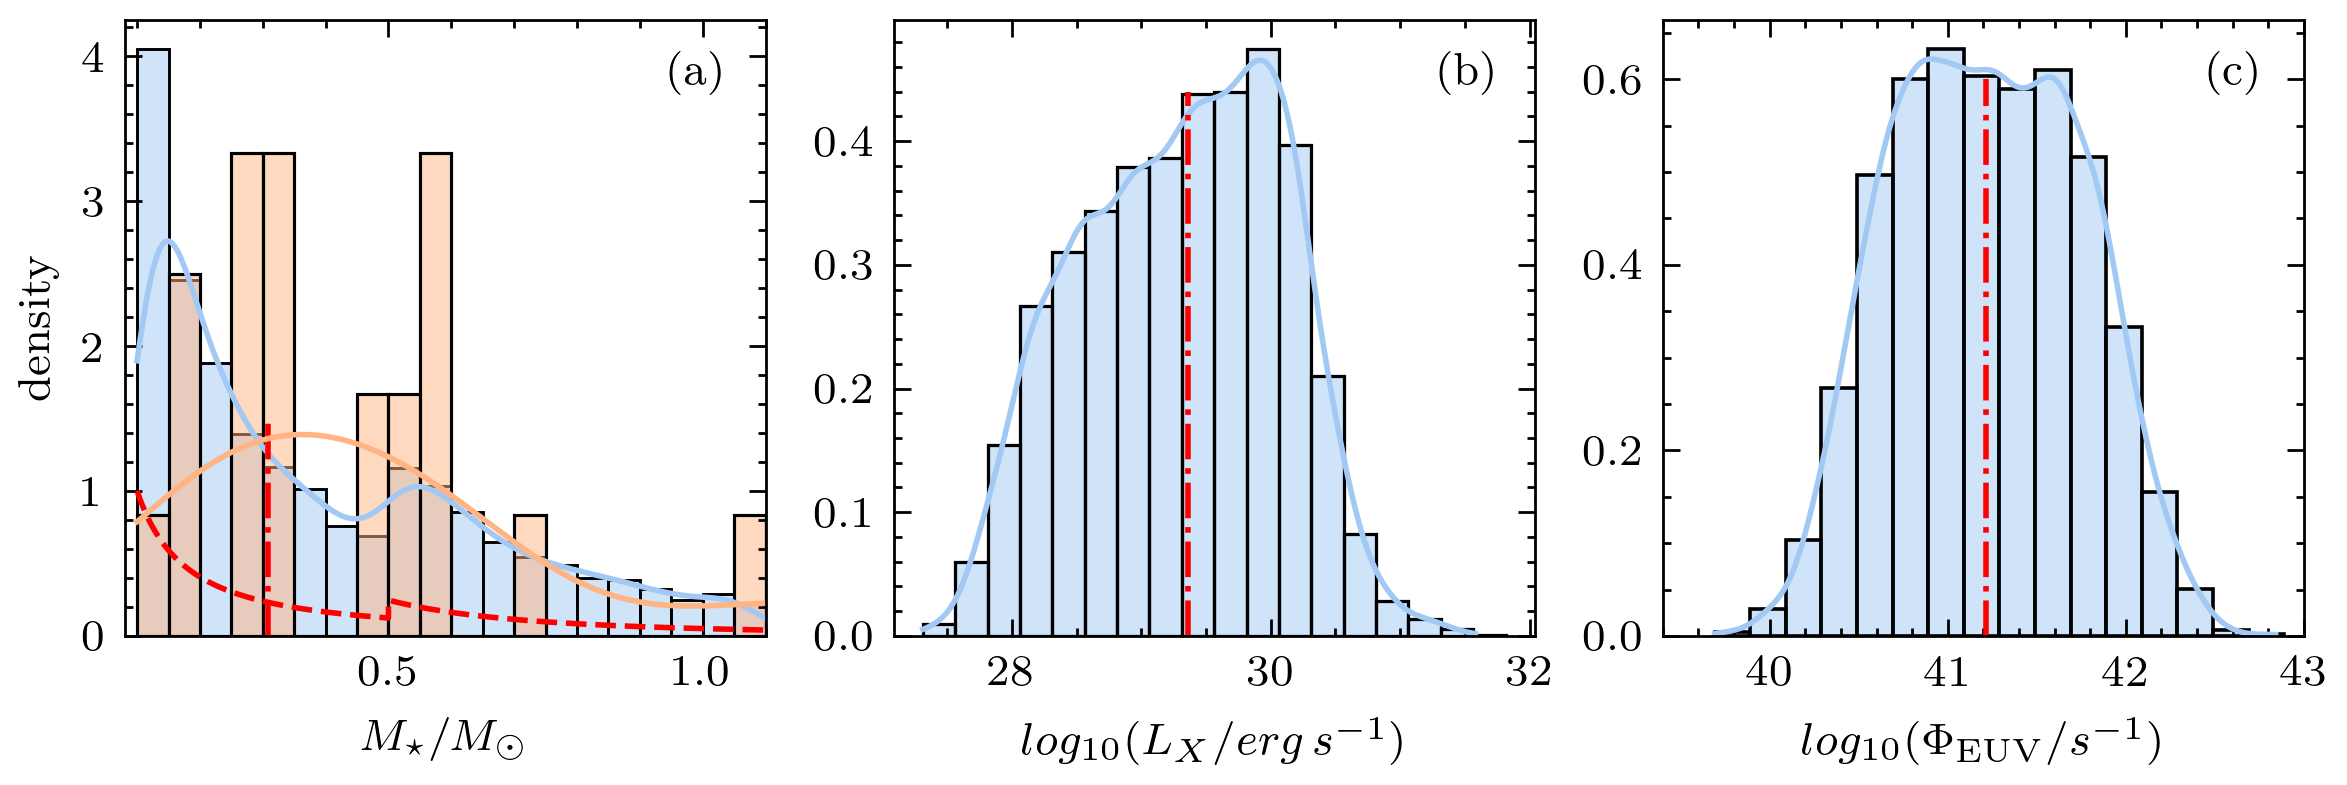
\includegraphics[width=\textwidth]{Fig1}
    \caption{Panel a: histogram of the stellar mass distribution in our population synthesis, where the KDE is overplotted with a blue solid line, the median value of $0.3$ M$_\odot$ is marked with a dotted-dashed red line, and the adopted weigthing based on the Kroupa IMF is plotted with a dashed red line. Panel b: histogram of the X-ray luminosity density distribution in the XEUV population synthesis, where the KDE is overplotted with a blue solid line and the median value of $29.4$ is marked with a dotted dashed red line. Panel c: histogram of the ionizing flux density distribution in the EUV population synthesis, where the KDE is overplotted with a blue solid line and the median value of $41.2$ is marked with a dotted dashed red line.\label{fig:hist}}
\end{figure*}

\citet{Gudel2007} derived an observational relation between the median X-ray luminosities and stellar masses
\begin{equation} \label{eq:LxMstar}
    \log_{10}(L_{X}) = (1.54\pm0.12) \log_{10}(M_\star) + (30.31\mp0.06) \,,
\end{equation}
though a large spread is observed around the mean values, which becomes larger for small mass stars \citep[e.g.][]{Getman2022}.
\citet{Kuhn2019} took a subsample of the Chandra Orion Ultradeep Project (\textsc{COUP}, \citet{Feigelson2005,Getman2005}) and stratified it in 3 stellar mass bins using the \citet{Baraffe1998} evolutionary models. From this sample one can derive a X-ray luminosity function (XLF) as a function of stellar mass.
%, as shown in Figure~\ref{fig:XLF}, from which one can see the increase in the median X-ray luminosity as a function of stellar mass as well as the increase spreading for lower stellar masses.
We then calculated the median stellar mass for the three stellar mass bins 
%in Figure~\ref{fig:XLF} 
given the adopted IMF, and shifted the XLF distribution to match the given value of the stellar mass. We sampled then the X-ray luminosity given the probability density corrected for the stellar mass and obtained the X-ray luminosity distribution shown in Figure~\ref{fig:hist} (panel b) from the 10,000 sampled stellar masses, with a median value of $10^{29.4}$ erg s$^{-1}$ and a spread over 4 orders of magnitude.
%\begin{figure}
%    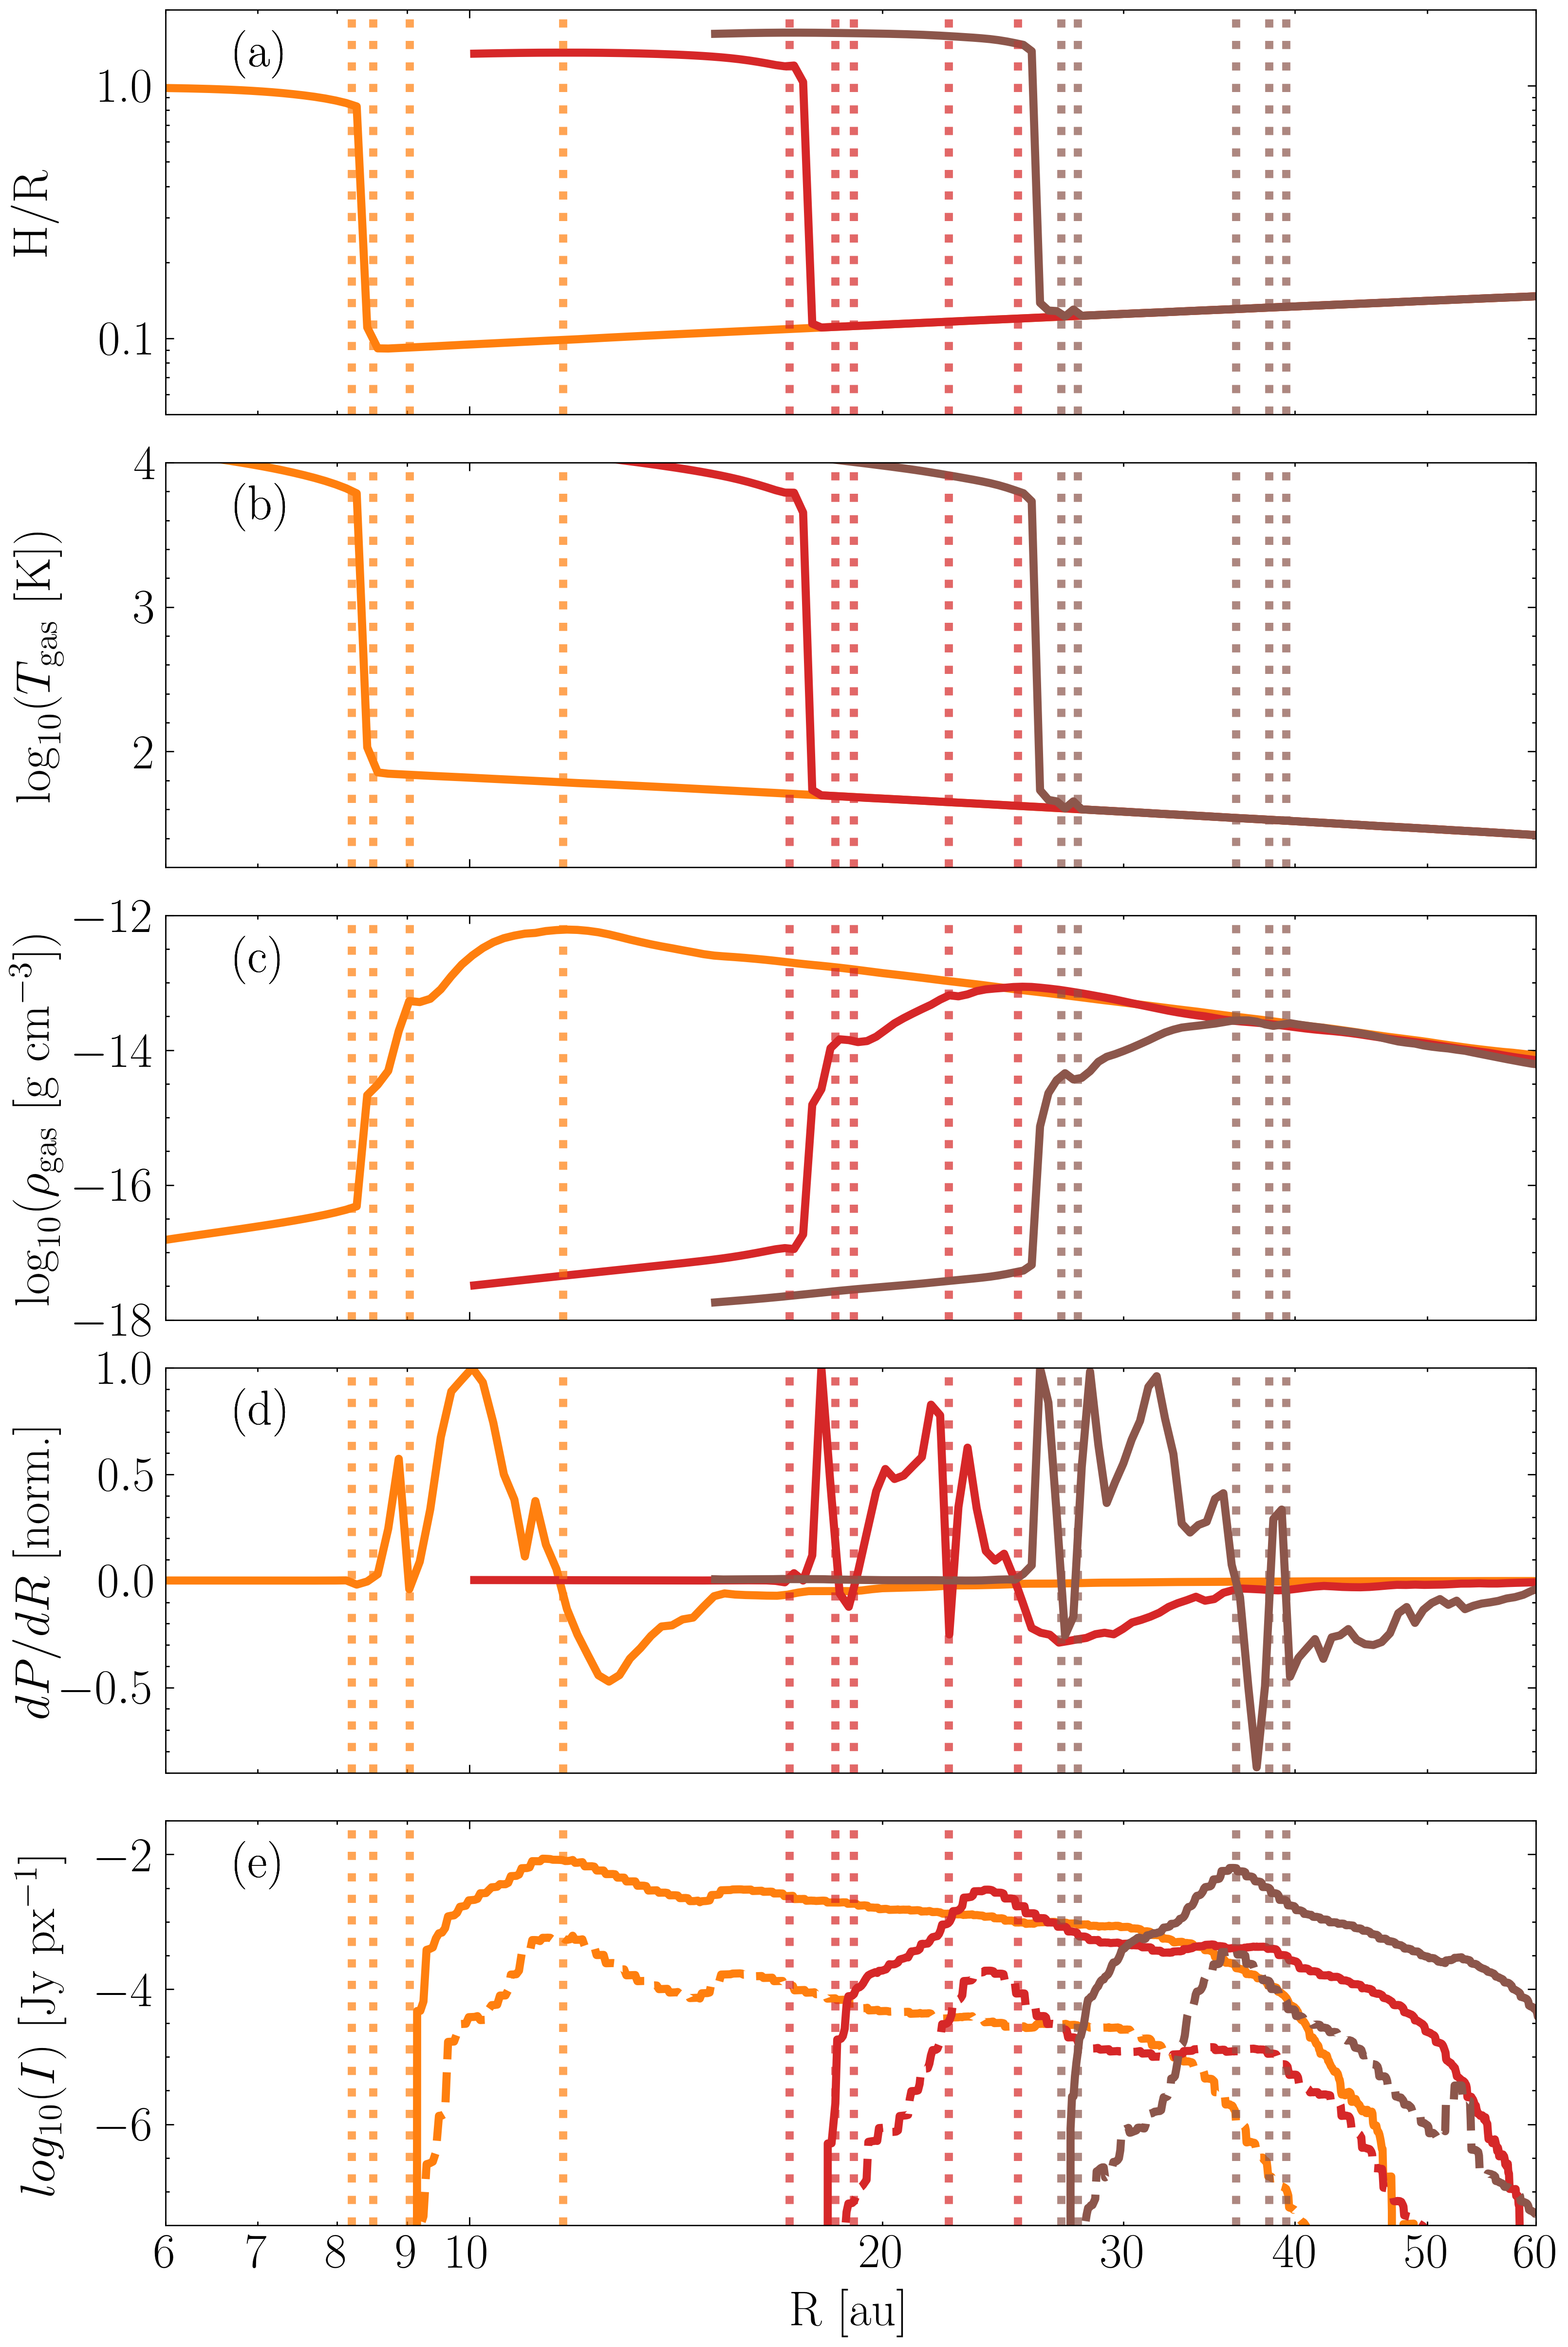
\includegraphics[width=\columnwidth]{Fig2}
%    \caption{X-ray luminosity function for a representative sample of generic young stellar objects sample of pre-main-sequence stars detected in the Chandra Orion Ultradeep Project (\textsc{COUP}; \citet{Feigelson2005,Getman2005}), stratified in 3 stellar mass bins as in \citet{Kuhn2019}. \label{fig:XLF}}
%\end{figure}
%\begin{figure}
%    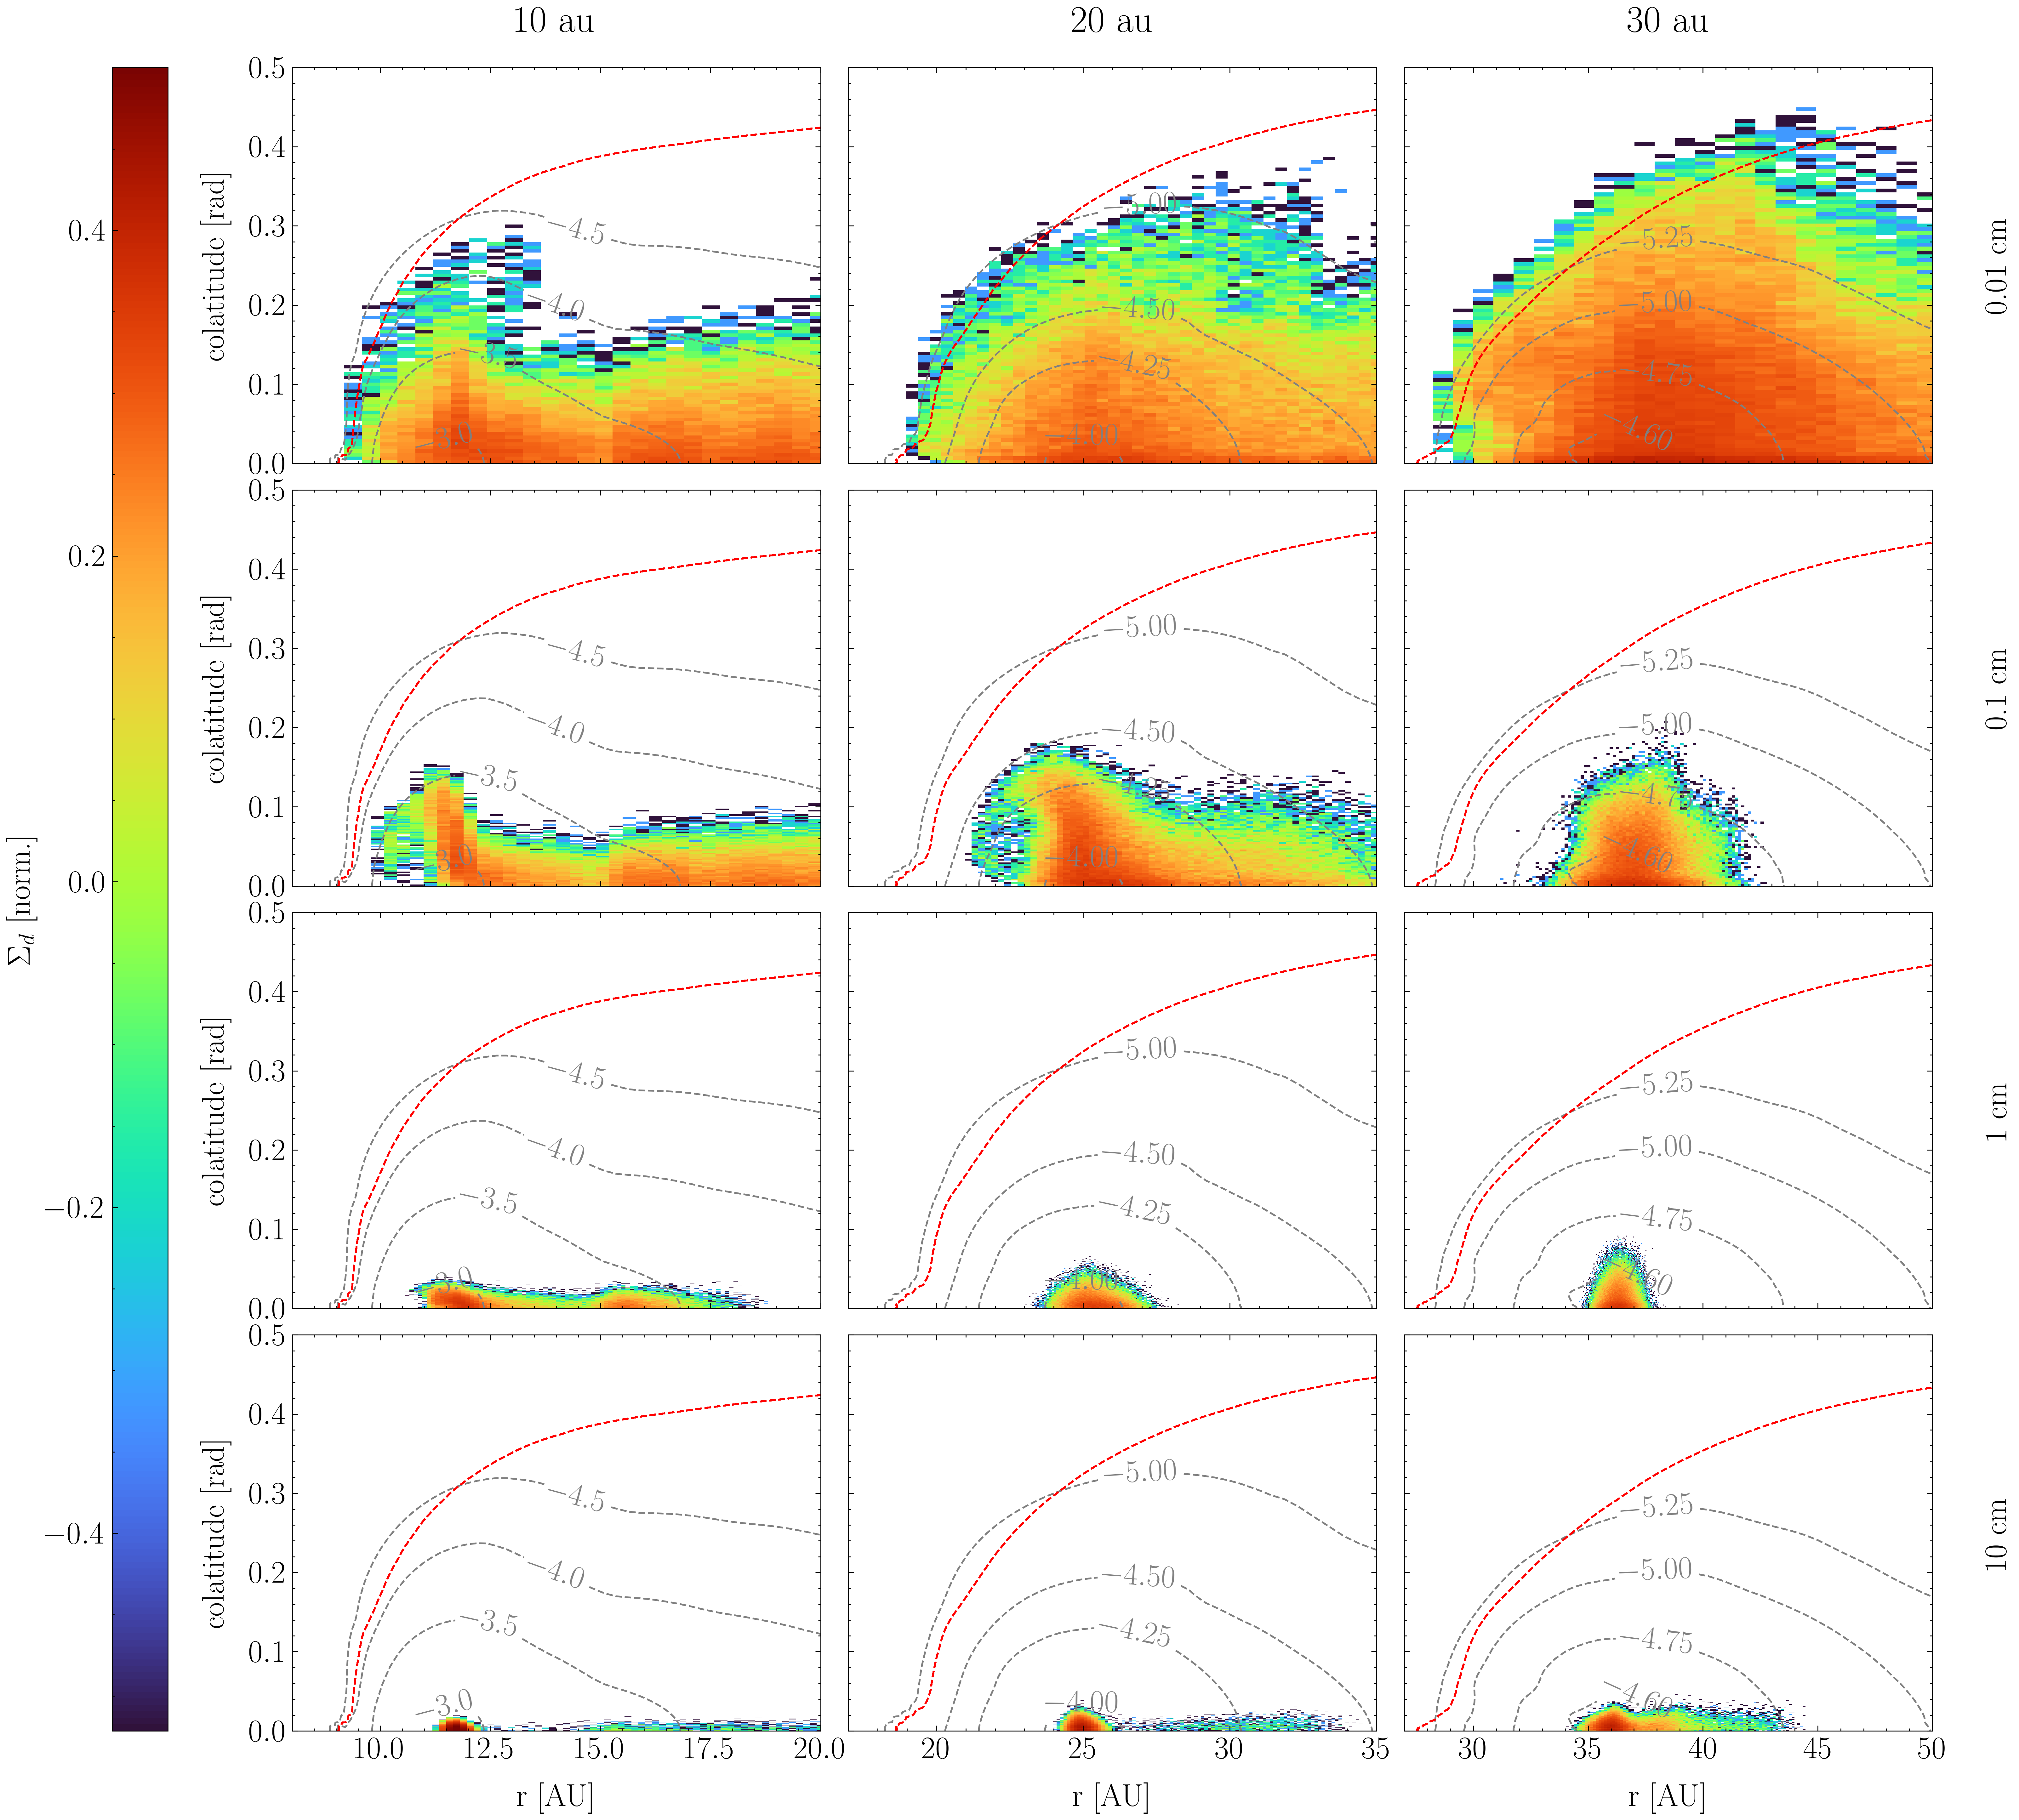
\includegraphics[width=\columnwidth]{Fig3}
%    \caption{Histogram of the X-ray luminosity density distribution in the XEUV population synthesis, where the KDE is overplotted with a dark blue solid line and the median value of 29.4 is marked with a dotted dashed black line. \label{fig:Lx}}
%\end{figure}

The EUV rates are shown to scale with the ratio of incoming ionising flux. However, there is no clear evidence on the origin of the EUV flux. Assuming that the EUV flux has the same origin as the X-ray flux we can then adopt the same scaling relation as eq.~\ref{eq:LxMstar}
\begin{equation} \label{eq:PhiEUVMstar}
    \log_{10}(\Phi_{EUV}) = 1.54 \log_{10}(M_\star) + 42 \,
\end{equation}
and adopt a small dispersion around the mean value for each stellar mass of 0.25 dex, as shown in Figure~\ref{fig:hist} (panel c), which gives a range of ionizing flux from $10^{40} s^{-1}$ to $10^{42.5} s^{-1}$ and a median value of $10^{41.2} s^{-1}$.
%\begin{figure}
%    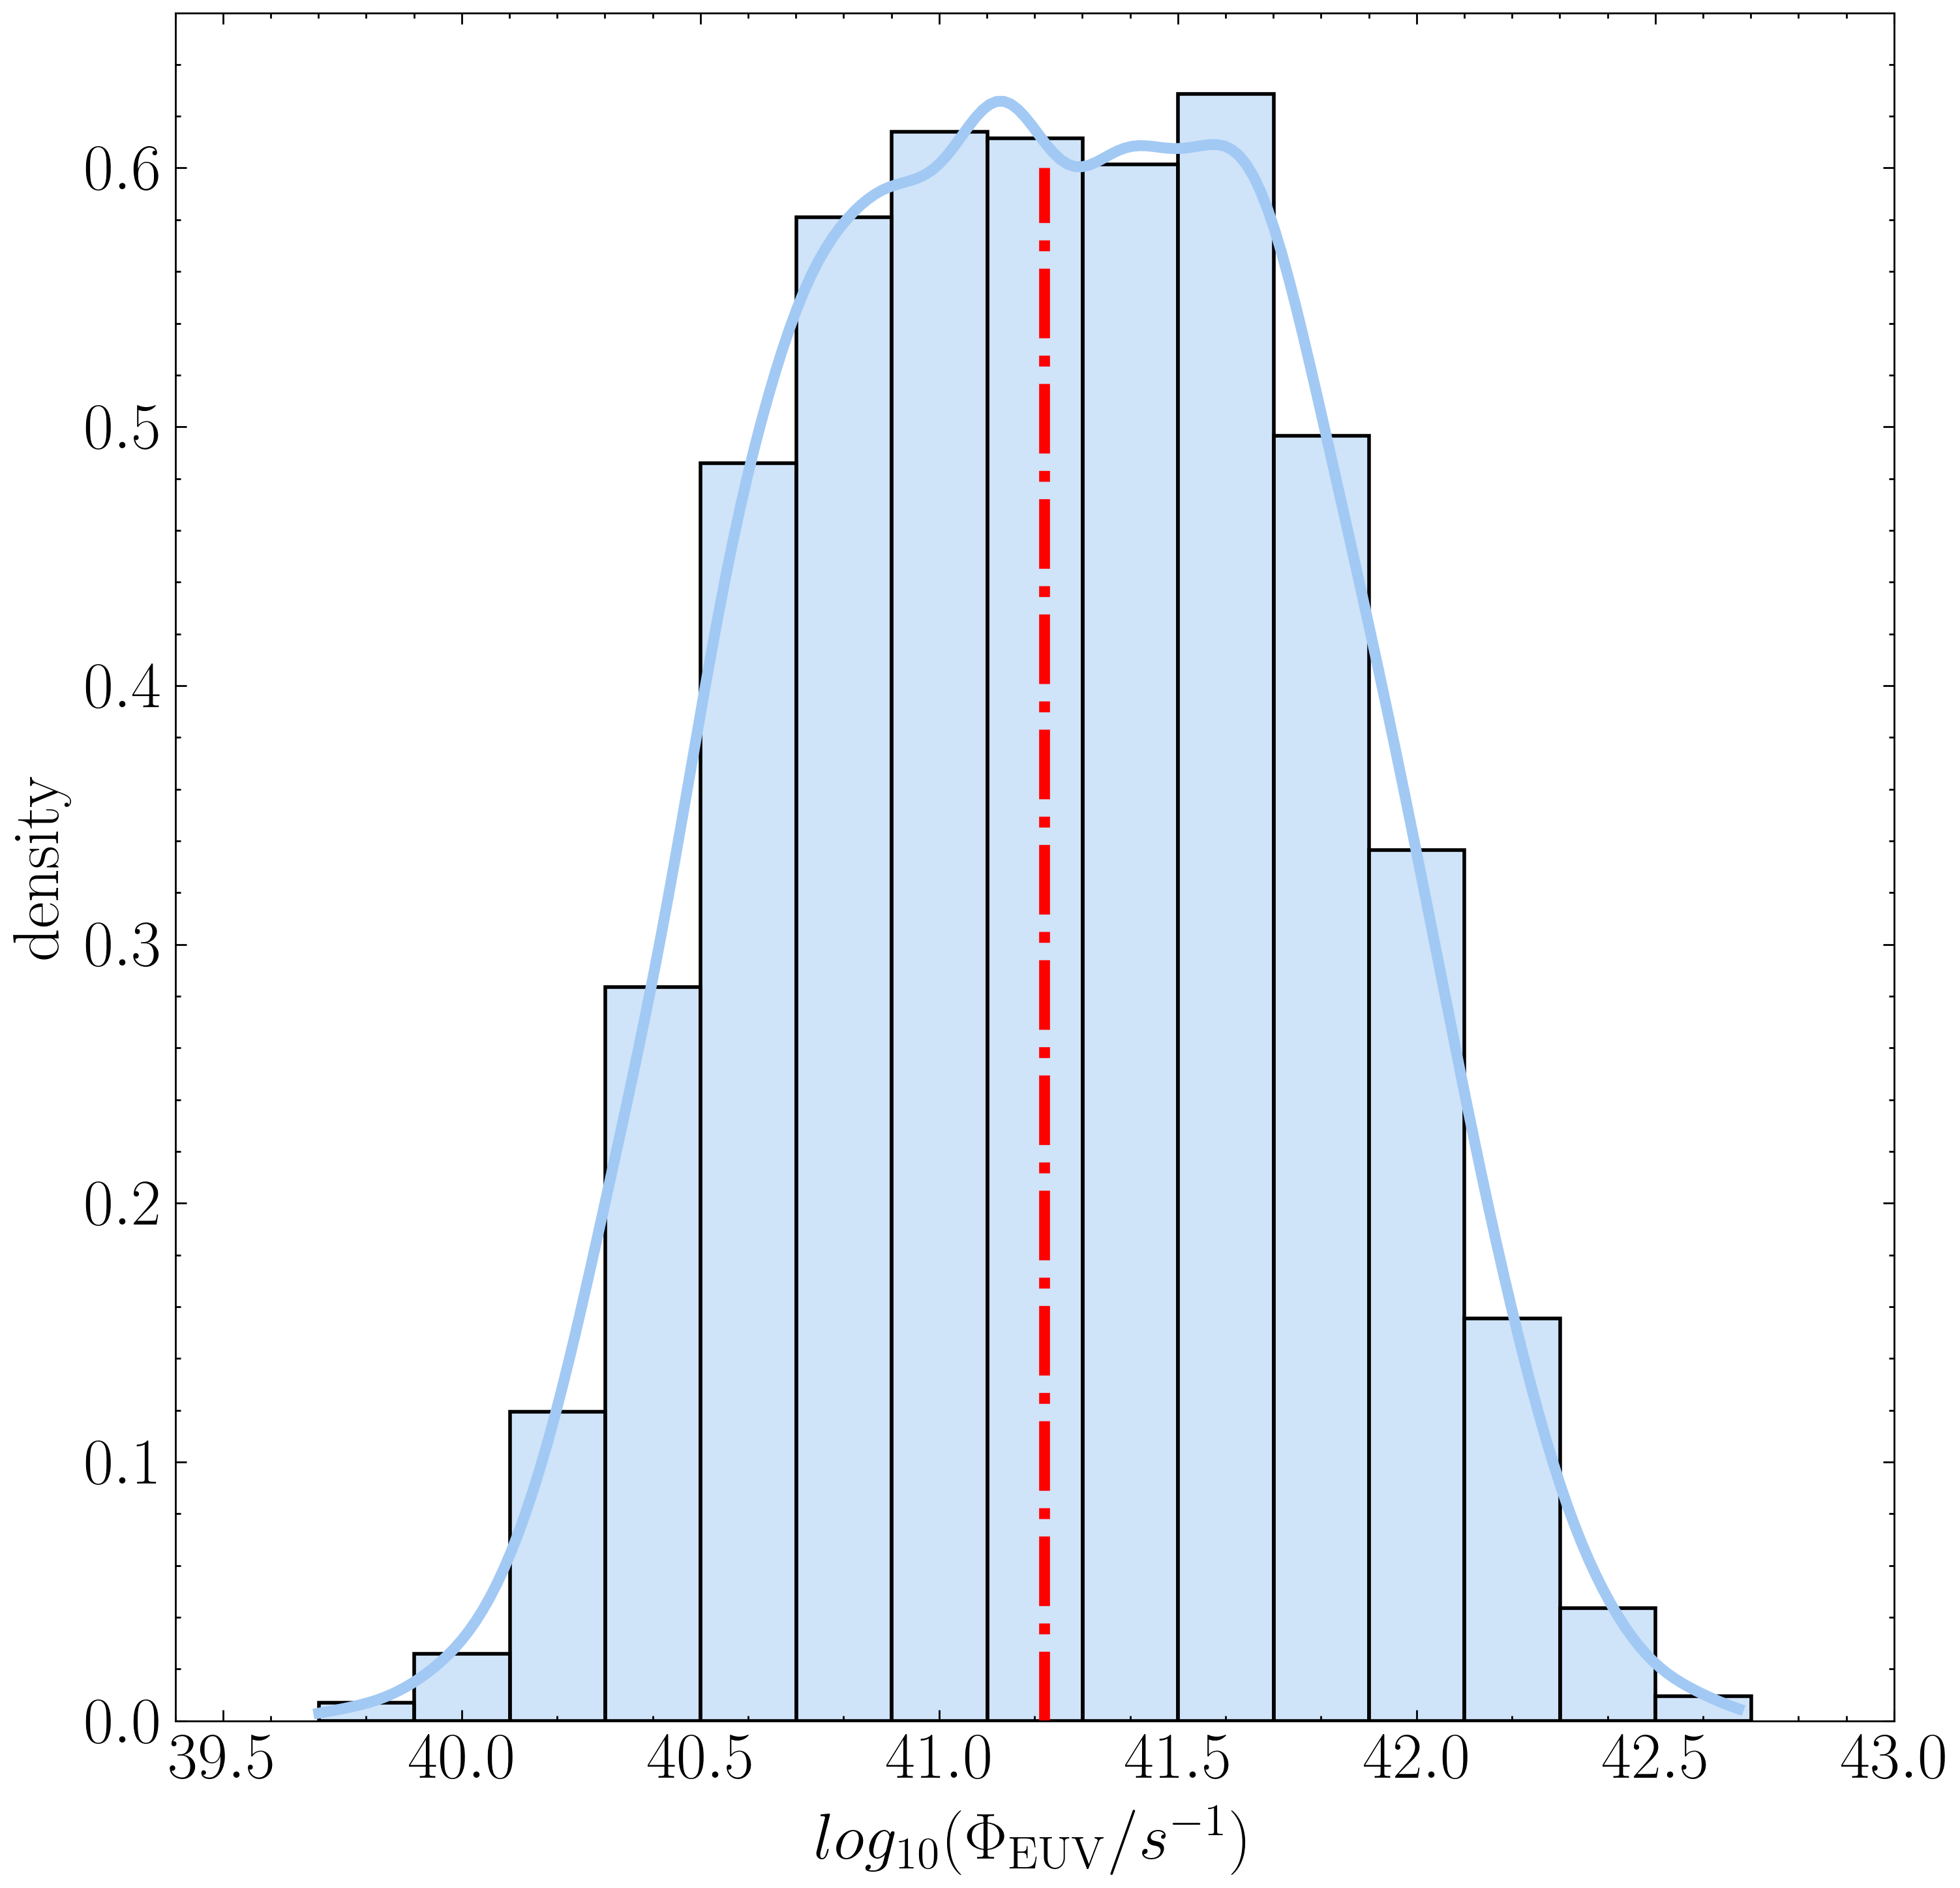
\includegraphics[width=\columnwidth]{Fig4}
%    \caption{Histogram of the ionizing flux density distribution in the EUV population synthesis, where the KDE is overplotted with a dark blue solid line and the median value of 41.2 is marked with a dotted dashed black line. \label{fig:phiEUV}}
%\end{figure}

We constrained the disc properties in order to match the observed mean disc lifetime of 2-3 Myr \citep[see e.g.][]{Ribas2014}. For the EUV profile we sampled the viscous $\alpha$ and scaling radius $R_1$ for disc masses ranging from $0.1$ to $0.01 M_\star$ for a typical star with median values from our distribution ($M_\star = 0.3 M_\odot$, $\Phi_\mathrm{EUV} = 10^{41.2}$ s$^{-1}$) and then we selected only the ones that were giving a correct disc life-time and obtained a best linear fit given by:
\begin{equation}\label{eq:r1_alpha}
    R_1 = 60.4 \alpha + 3009.7 M_d [M_\star] + 226.6 \\\text{[au]} \,.
\end{equation}
We then sampled the whole stellar mass range and obtained the full sampling of the parameter space.
%shown in Figure~\ref{fig:param_euv}.
%\begin{figure*}
%    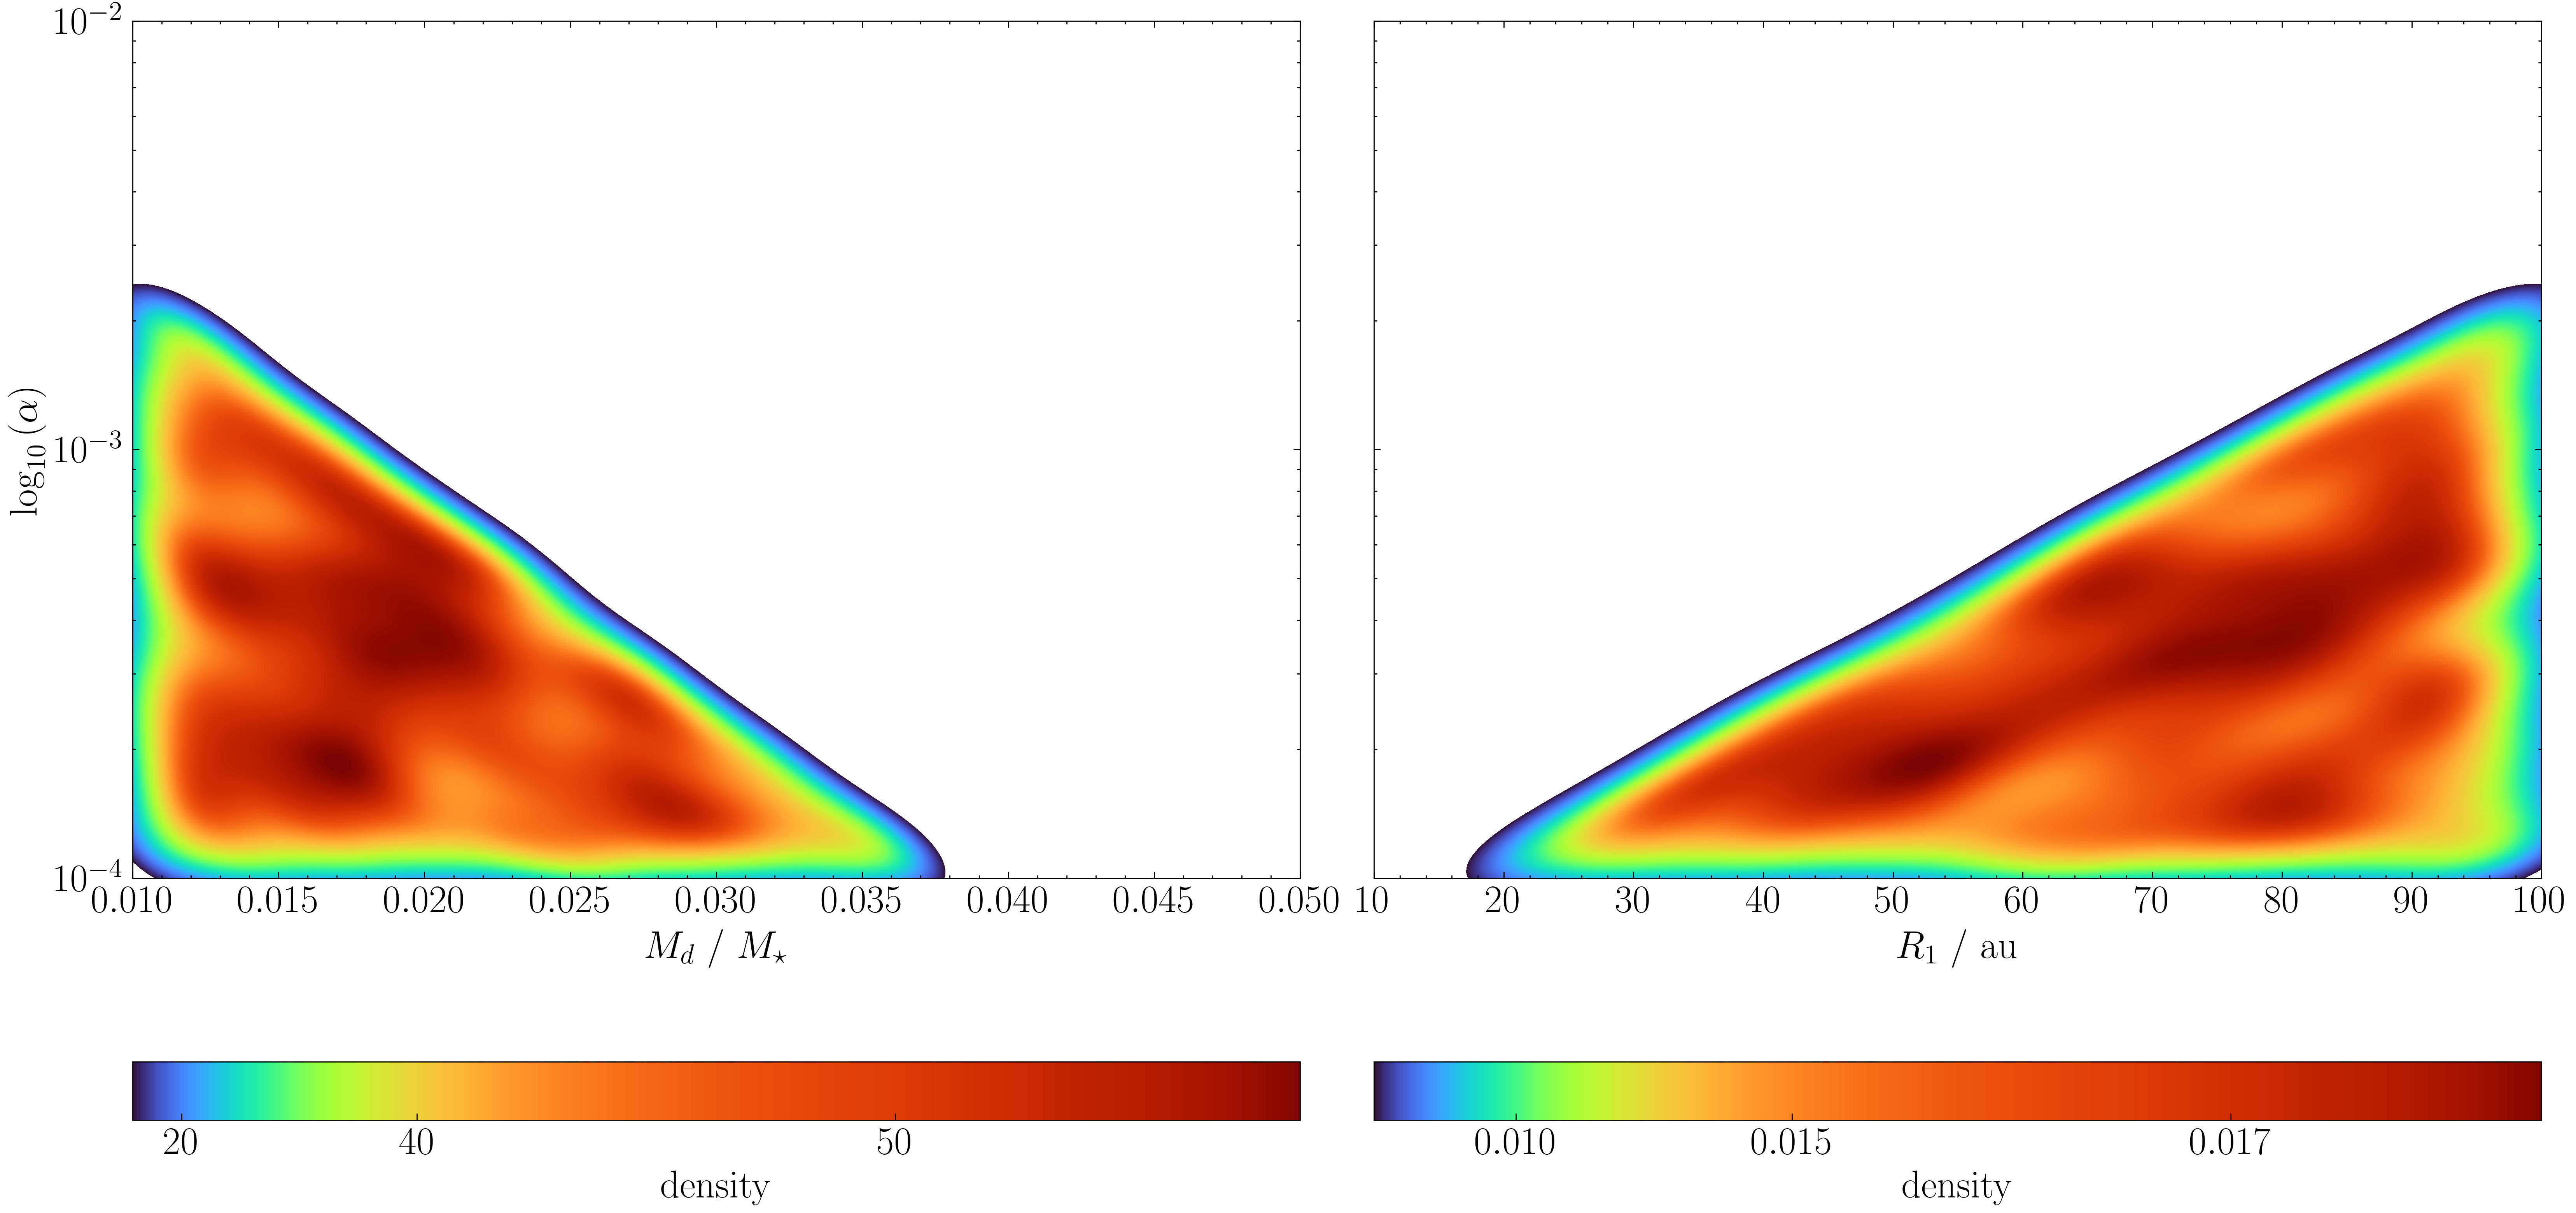
\includegraphics[width=0.92\textwidth]{Fig5}
%    \caption{KDE plot of the alpha - disc mass (left) and alpha-r1 (right) parameters that were adopted in the EUV population synthesis in order to have a disc life-time compatible with the observationally derived one. \label{fig:param_euv}}
%\end{figure*}
For the XEUV profile we realized that the disc evolution was primarily driven by the internal photoevaporation rather than the disc properties, thus we chose to sample uniformly the parameter space for the disc properties and fix only the disc mass to $0.1 M_\star$ as this is a reasonable value of the initial disc mass when the disc self-gravity stops being the driver of disc evolution and the approximation of a viscously evolving disc is reasonable. We summarize the parameter space probed in Table~\ref{tab:popsynthtable}.
\begin{table*}
	\centering
	\caption{Parameters for the population synthesis calculations.}
	\label{tab:popsynthtable}
	\begin{tabular}{lccccr}
        \hline
		\hline
		  name & viscosity & r1 & disc mass & stellar mass & stellar flux \\
        & $\log_{10}(\alpha)$ & au & $M_\star$ & $M_\odot$ & $(\Phi_{EUV},\ L_X)$\\
		\hline
		  EUV & eq.~\ref{eq:r1_alpha} & eq.~\ref{eq:r1_alpha} & eq.~\ref{eq:r1_alpha} & Fig.~\ref{fig:hist} (panel a) & Fig.~\ref{fig:hist} (panel c)\\
		XEUV & [-4, -2] & [10, 100] & 0.1 & Fig.~\ref{fig:hist} (panel a) & Fig.~\ref{fig:hist} (panel b)\\
		%3 & 5 & 7 & 9\\
		\hline
	\end{tabular}
\end{table*}

\section{Results}\label{sec:results}

Figure~\ref{fig:mdot_age} shows the accretion rates as a function of time for a population synthesis of 10,000 discs sampled as described in the previous section.
Overplotted with dots of variable size (based on their stellar mass) is the population of low accretors from \citet{Thanathibodee2023}, and the observational limit of the He I $\lambda10830$ marked with a black dashed line at $10^{-11}$ M$_\odot$ yr$^{-1}$.
One can immediately see that while the XEUV profile catches all the observed data points in the region with high density ($> 10^{-2}$), the EUV cannot explain the data for the older star-forming regions (Orion OB1a and Upper Sco). Furthermore the observational data points lie in the upper region of the distribution, even though they are a sample of the low-accretors population. This means that the bulk of the discs in the studied star forming regions covers a region not explained by the EUV photoevaporation profiles.
\begin{figure*}
    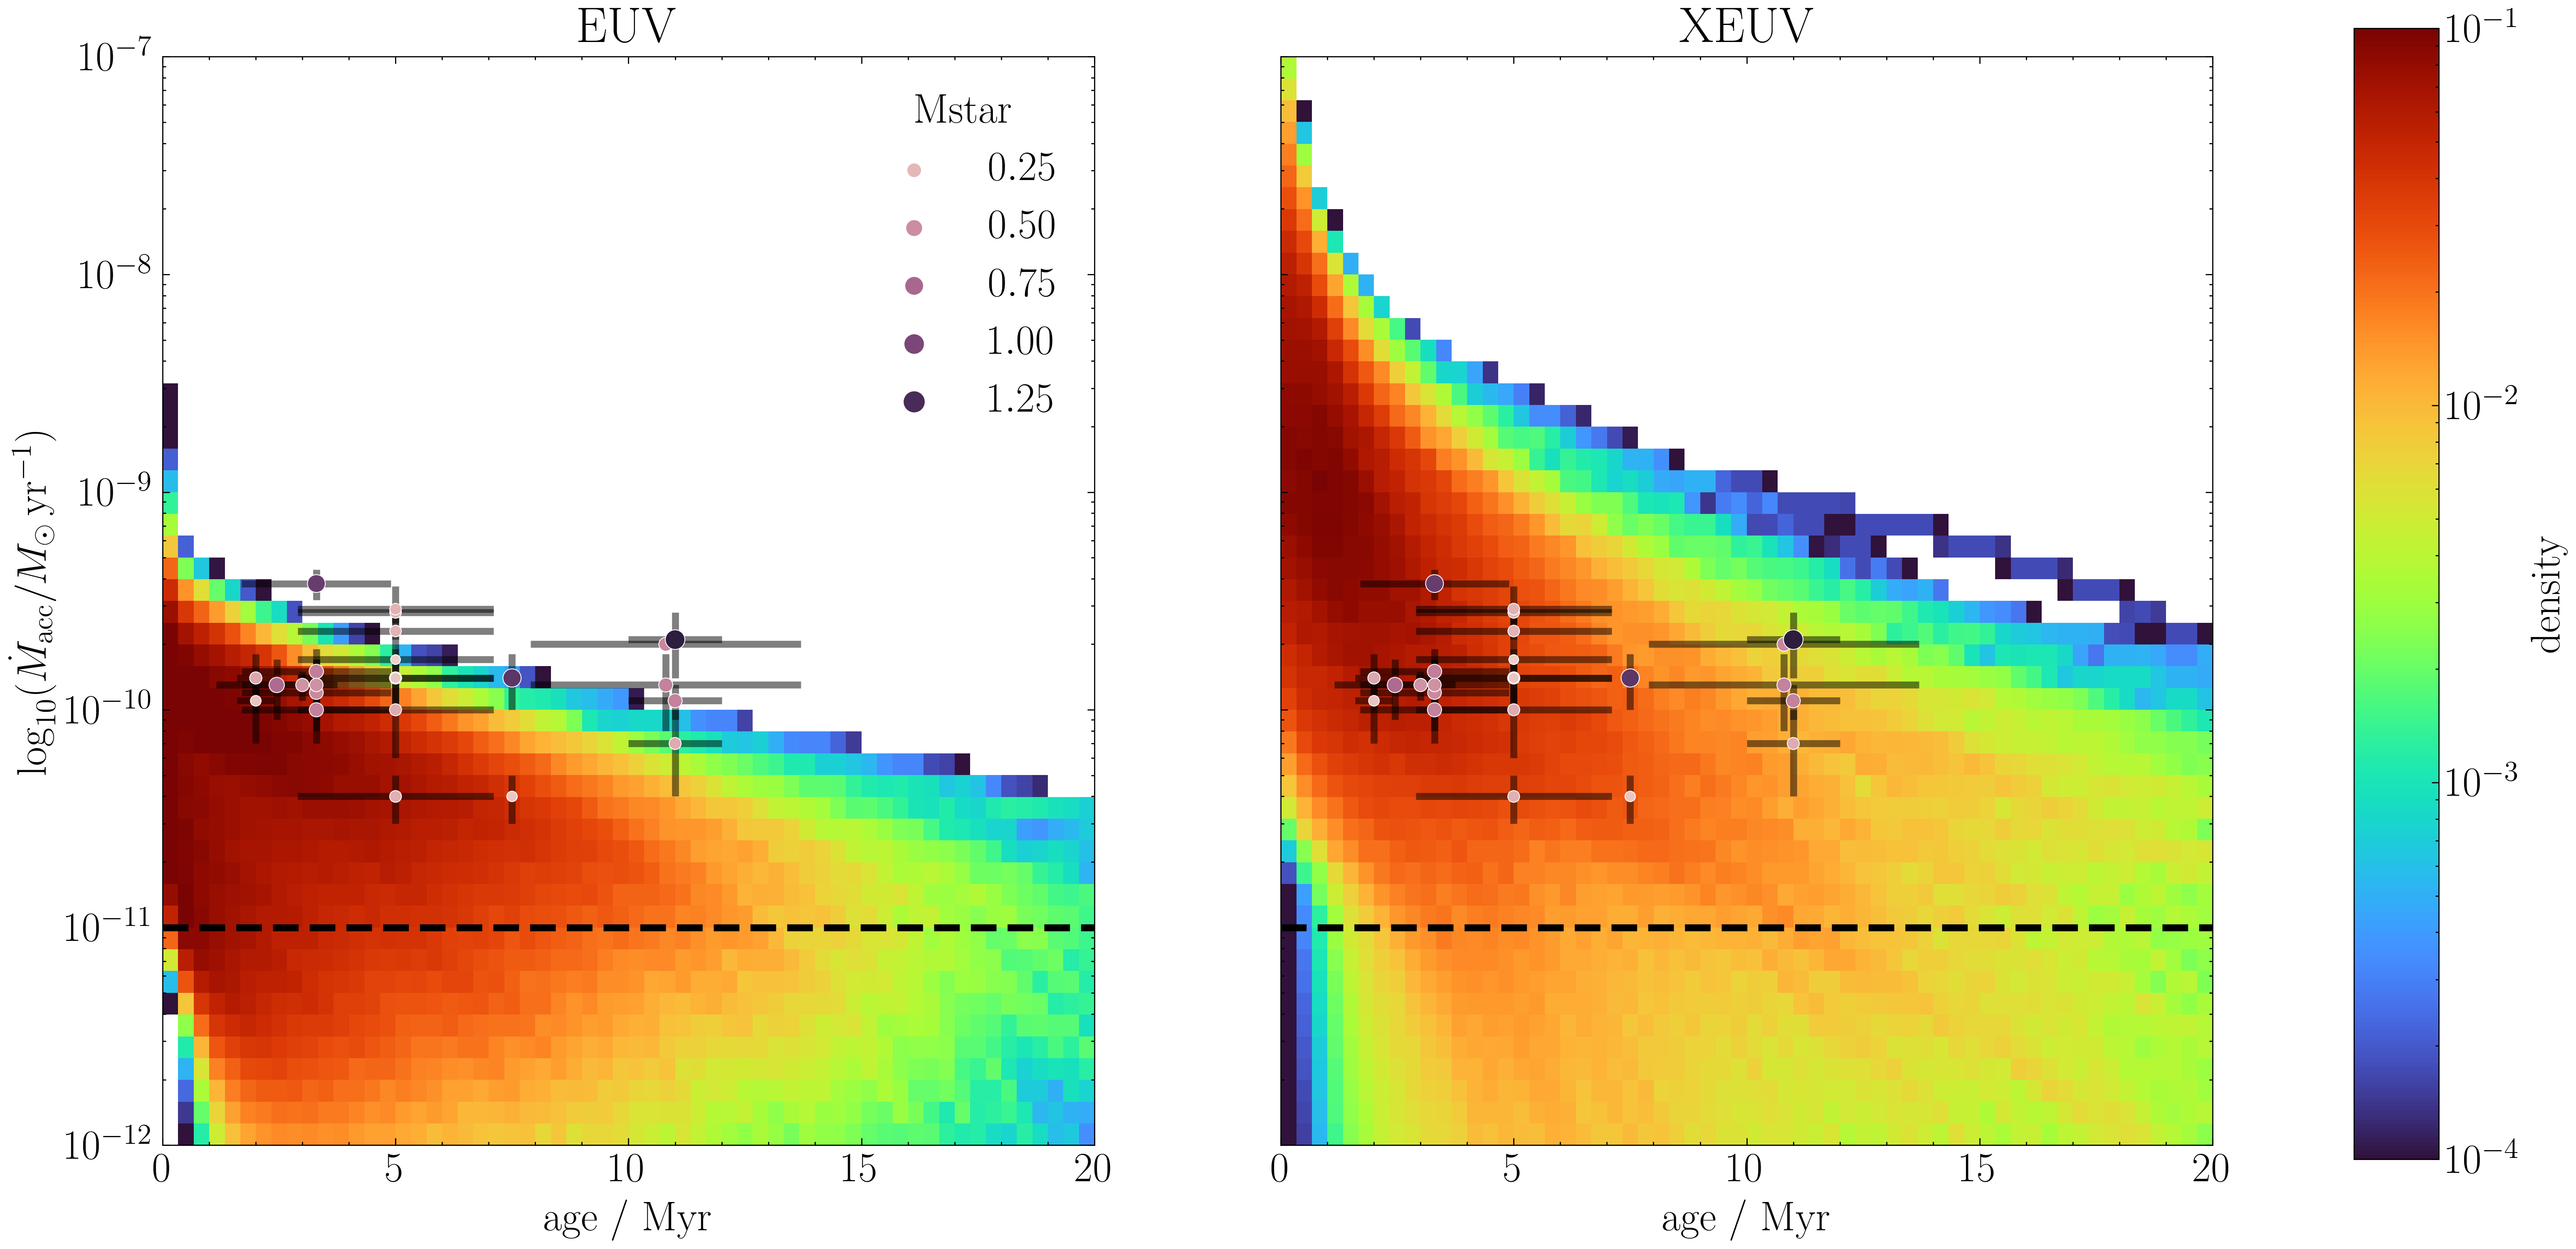
\includegraphics[width=0.92\textwidth]{Fig6}
    \caption{Synthetic populations showing the accretion rates as a function of age. The color mapping shows the probability of finding an object of a given age accreting at a given accretion rate (see text for details). Left panel: discs are dispersed by EUV photoevaporation; right panel: discs are dispersed by X-ray photoevaporation. The low-accretors population is overplotted with dots with variable size increasing by their stellar mass.
    \label{fig:mdot_age}}
\end{figure*}

%Another way to show the results, and avoid the errors related to the %age determination of star forming regions is to plot the accretion rates as a function of the star forming region disc fractions (see Figure~\ref{fig:mdot_frac}). In a similar way here the data points for the low-accretors lie all in the region with low probability density or not explained by the current EUV models (left panel). The situation is significantly different looking at the XEUV population (right panel) where the data points sit in the bulk of the distribution.
Small mass stars (small dots) cover the lower part of the high density distribution while bigger stars the top part. This is expected from the observationally derived relation between accretion rate and stellar masses, that shows a sharp increase of the accretion rate as a function of stellar mass with a broken power law \citep{Alcala2017}.

%\begin{table*}
%	\centering
%	\caption{Observational properties of the low-accretors population.\\ \note{(1) \citet{Thanathibodee2023}, (2) \citet{daRio2016}, (3) \citet{Galli2021}, (4) \citet{Briceno2019}}}
%	\label{tab:low-acretors-table}
%	\begin{tabular}{lcccccr} % four columns, alignment for each
%		\hline
%		  Group & Age & Disc Fraction & Target & Stellar mass & Accretion rate & References \\
%         & (Myr) & (\%) & & M$_\odot$ & ($10^{-10}$ M$_\odot$ yr$^{-1}$) & \\
%		\hline
%        \hline
%        \multirow{2}{*}{OriOB1a} & \multirow{2}{*}{$10.8\pm2.9$} & \multirow{2}{*}{6} & CVSO 40 & 0.53 & $2.0\pm0.0$ & (1,4)\\
%        & & & CVSO 298 & 0.56 & $1.3\pm0.5$ & (1,4)\\
%        \hline
%        \multirow{8}{*}{OriOB1b} & \multirow{8}{*}{$5.0\pm2.1$} & \multirow{8}{*}{$12$} & CVSO 156 & 0.34 & $1.4\pm0.4$ & (1,4)\\
%        & & & CVSO 1545 & $0.17$ & $1.4\pm0.4$ & (1,4)\\
%        & & & CVSO 1600E & $0.27$ & $2.3\pm0.5$ & (1,4)\\
%        & & & CVSO 1600W & $0.27$ & $2.8\pm0.3$ & (1,4)\\
%        & & & CVSO 1739 & $0.10$ & $1.7\pm0.2$ & (1,4)\\
%        & & & CVSO 1772 & $0.29$ & $0.4\pm0.1$ & (1,4)\\
%        & & & CVSO 1842 & $0.32$ & $1.0\pm0.4$ & (1,4)\\
%        & & & CVSO 1886 & $0.28$ & $2.9\pm0.8$ & (1,4)\\
%        \hline
%        \multirow{5}{*}{Ori Cloud A} & \multirow{5}{*}{$3.3\pm1.6$} & \multirow{5}{*}{$28$} & CVSO 1295 & 0.59 & $1.5\pm0.4$ & (1,2,4)\\
%        & & & CVSO 1575 & 0.57 & $1.0\pm0.2$ & (1,2,4)\\
%        & & & CVSO 1711 & 0.52 & $1.2\pm0.5$ & (1,2,4)\\
%        & & & CVSO 1763 & 1.09 & $3.8\pm0.6$ & (1,2,4)\\
%        & & & CVSO 1928 & 0.47 & $1.3\pm0.4$ & (1,2,4)\\
%        \hline
%        Ori Cloud B & $2.45\pm1.3$ & $31$ & CVSO 1942 & 0.72 & $1.3\pm0.4$ & (1,4)\\
%        \hline
%        \multirow{2}{*}{Chamaeleon I} & \multirow{2}{*}{$2\pm0.4$} & \multirow{2}{*}{$44$} & ISO-ChaI 52 & 0.18 & $1.1\pm0.4$ & (1,3)\\
%        & & & CHSM 13620 & 0.34 & $1.4\pm0.4$ & (1,3)\\
%        \hline
%        \multirow{3}{*}{Upper Sco} & \multirow{3}{*}{10-12} & \multirow{3}{*}{$21\pm1$} & J16020757 & 0.32 & $0.7\pm0.3$ & (1)\\
%        & & & J16253849 & 0.56 & $1.1\pm0.2$ & (1)\\
%        & & & J16042165 & 1.39 & $2.1\pm0.7$ & (1)\\
%        \hline
%        \multirow{2}{*}{$\gamma$Vel} & \multirow{2}{*}{$7.5$} & \multirow{2}{*}{$6$} & J08074647 & 0.16 & $0.4\pm0.1$ & (1)\\
%        & & & J08075546 & 1.15 & $1.4\pm0.4$ & (1)\\
%        \hline
%        $\sigma$Ori & $3$ & $36\pm4$ & SO682 & 0.46 & $1.3\pm0.2$ & (1)\\
%		\hline
%	\end{tabular}
%\end{table*}
%\begin{figure*}
%    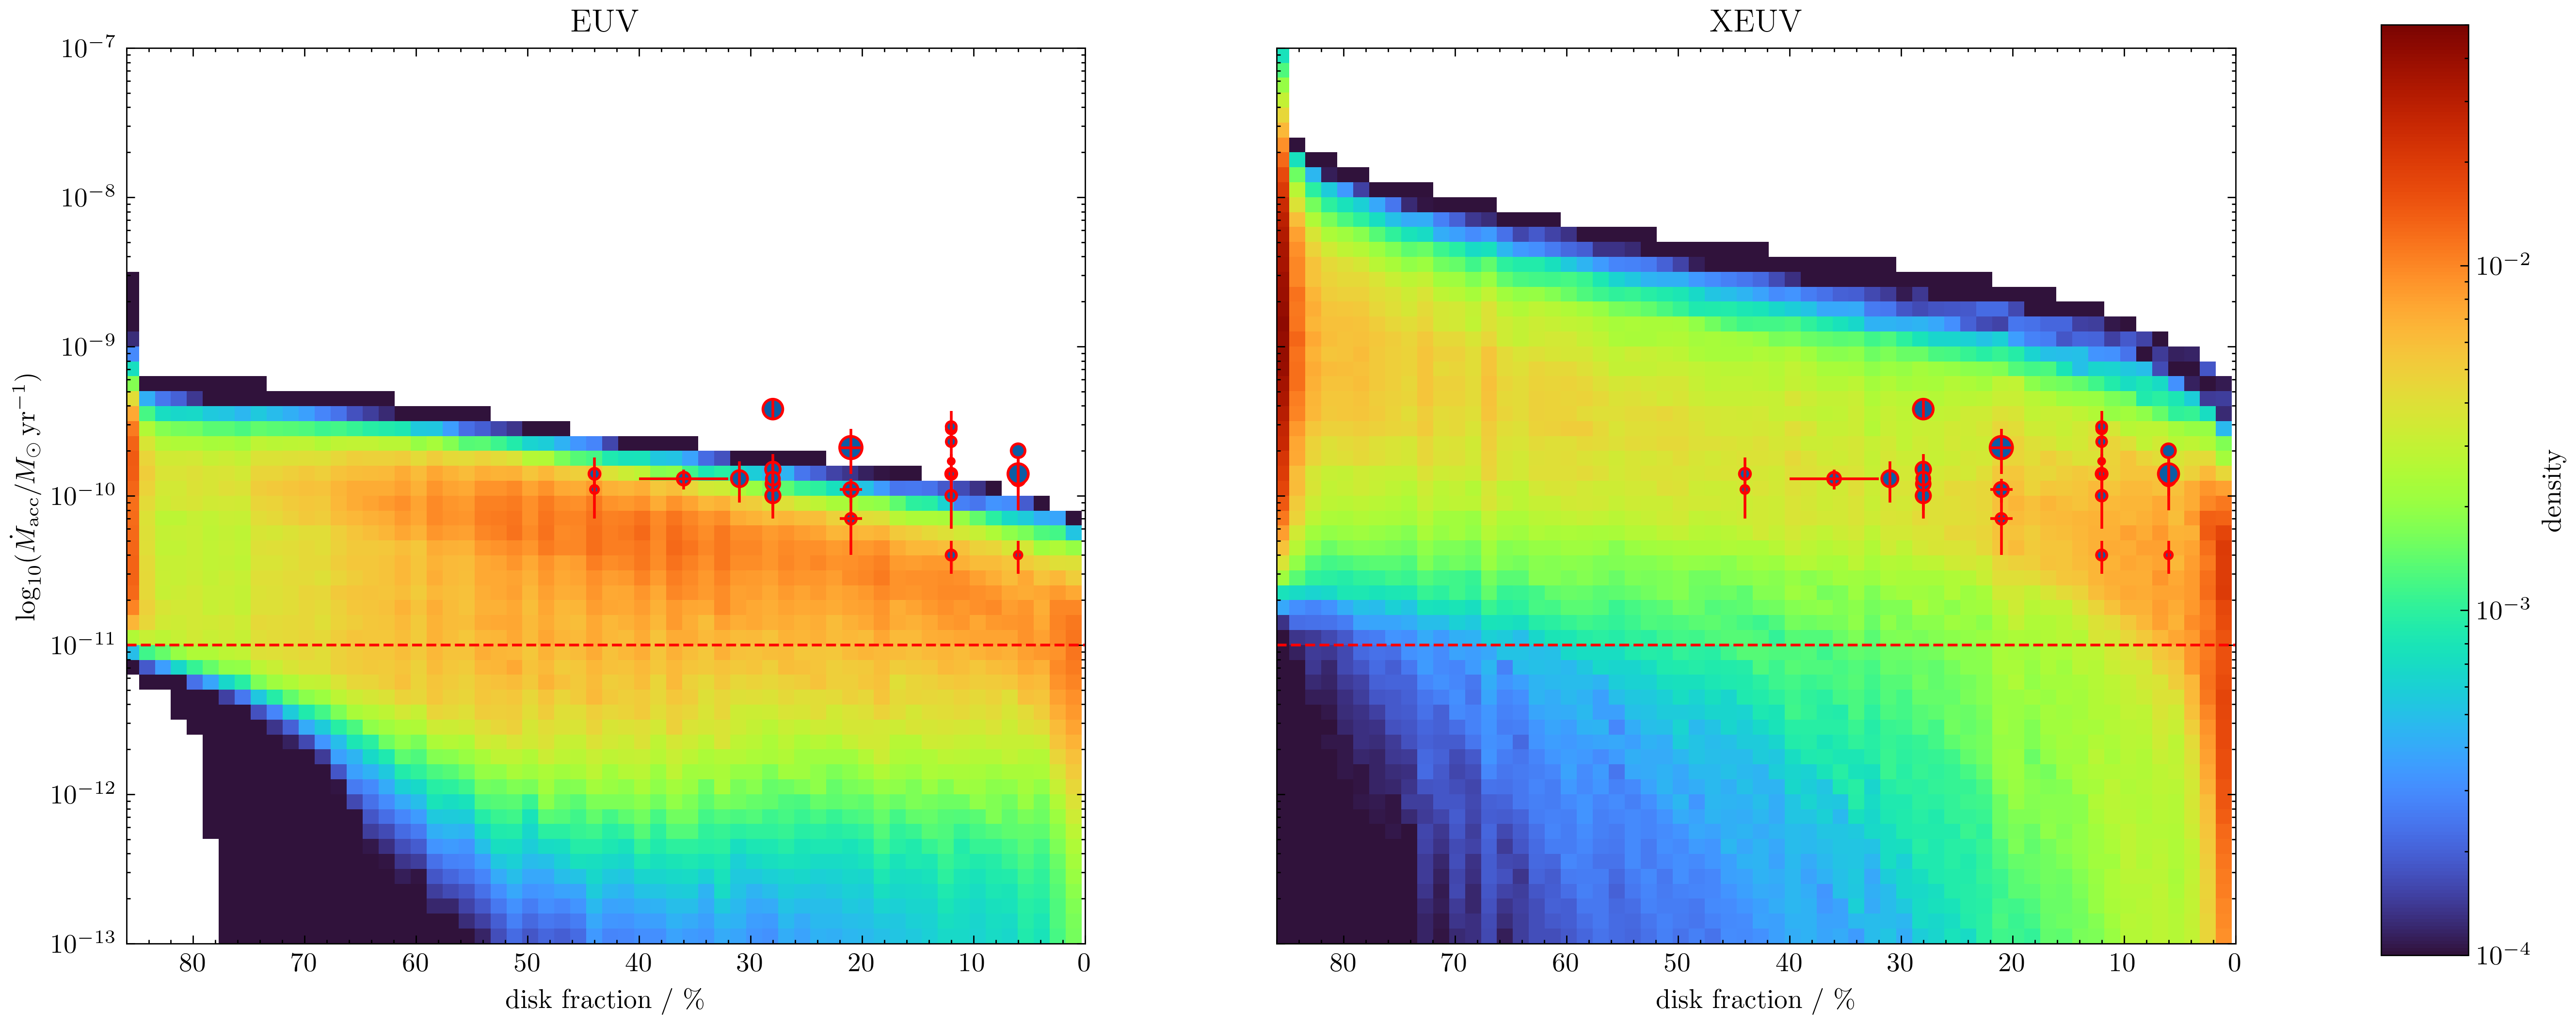
\includegraphics[width=0.92\textwidth]{mdot_frac_comparison}
%    \caption{Synthetic populations showing the accretion rates as a function of disc fraction. The colors show the probability of finding a disc of a given accretion rate in a star forming region with a given disc fraction (see text for details). Left panel: Discs are dispersed by EUV photoevaporation; right panel: discs are dispersed by X-ray photoevaporation. The low-accretors population is overplotted with blue dots with variable size increasing by the stellar mass.
%    \label{fig:mdot_frac}}
%\end{figure*}

We plotted in Figure~\ref{fig:hist_mdot} the histogram of the accretion rate distribution for the EUV (in blue) and XEUV (in orange) populations. We overplotted as well the median accretion rates in dotted-dashed blue and orange line respectively, and the median accretion rate for the observed population of low-accretors with a dotted-dashed black line. From this one can directly visualize how the median of the XEUV population and the observed low-accretors is very similar, while it is close to the high-accretor wing of the EUV distribution.
\begin{figure}
    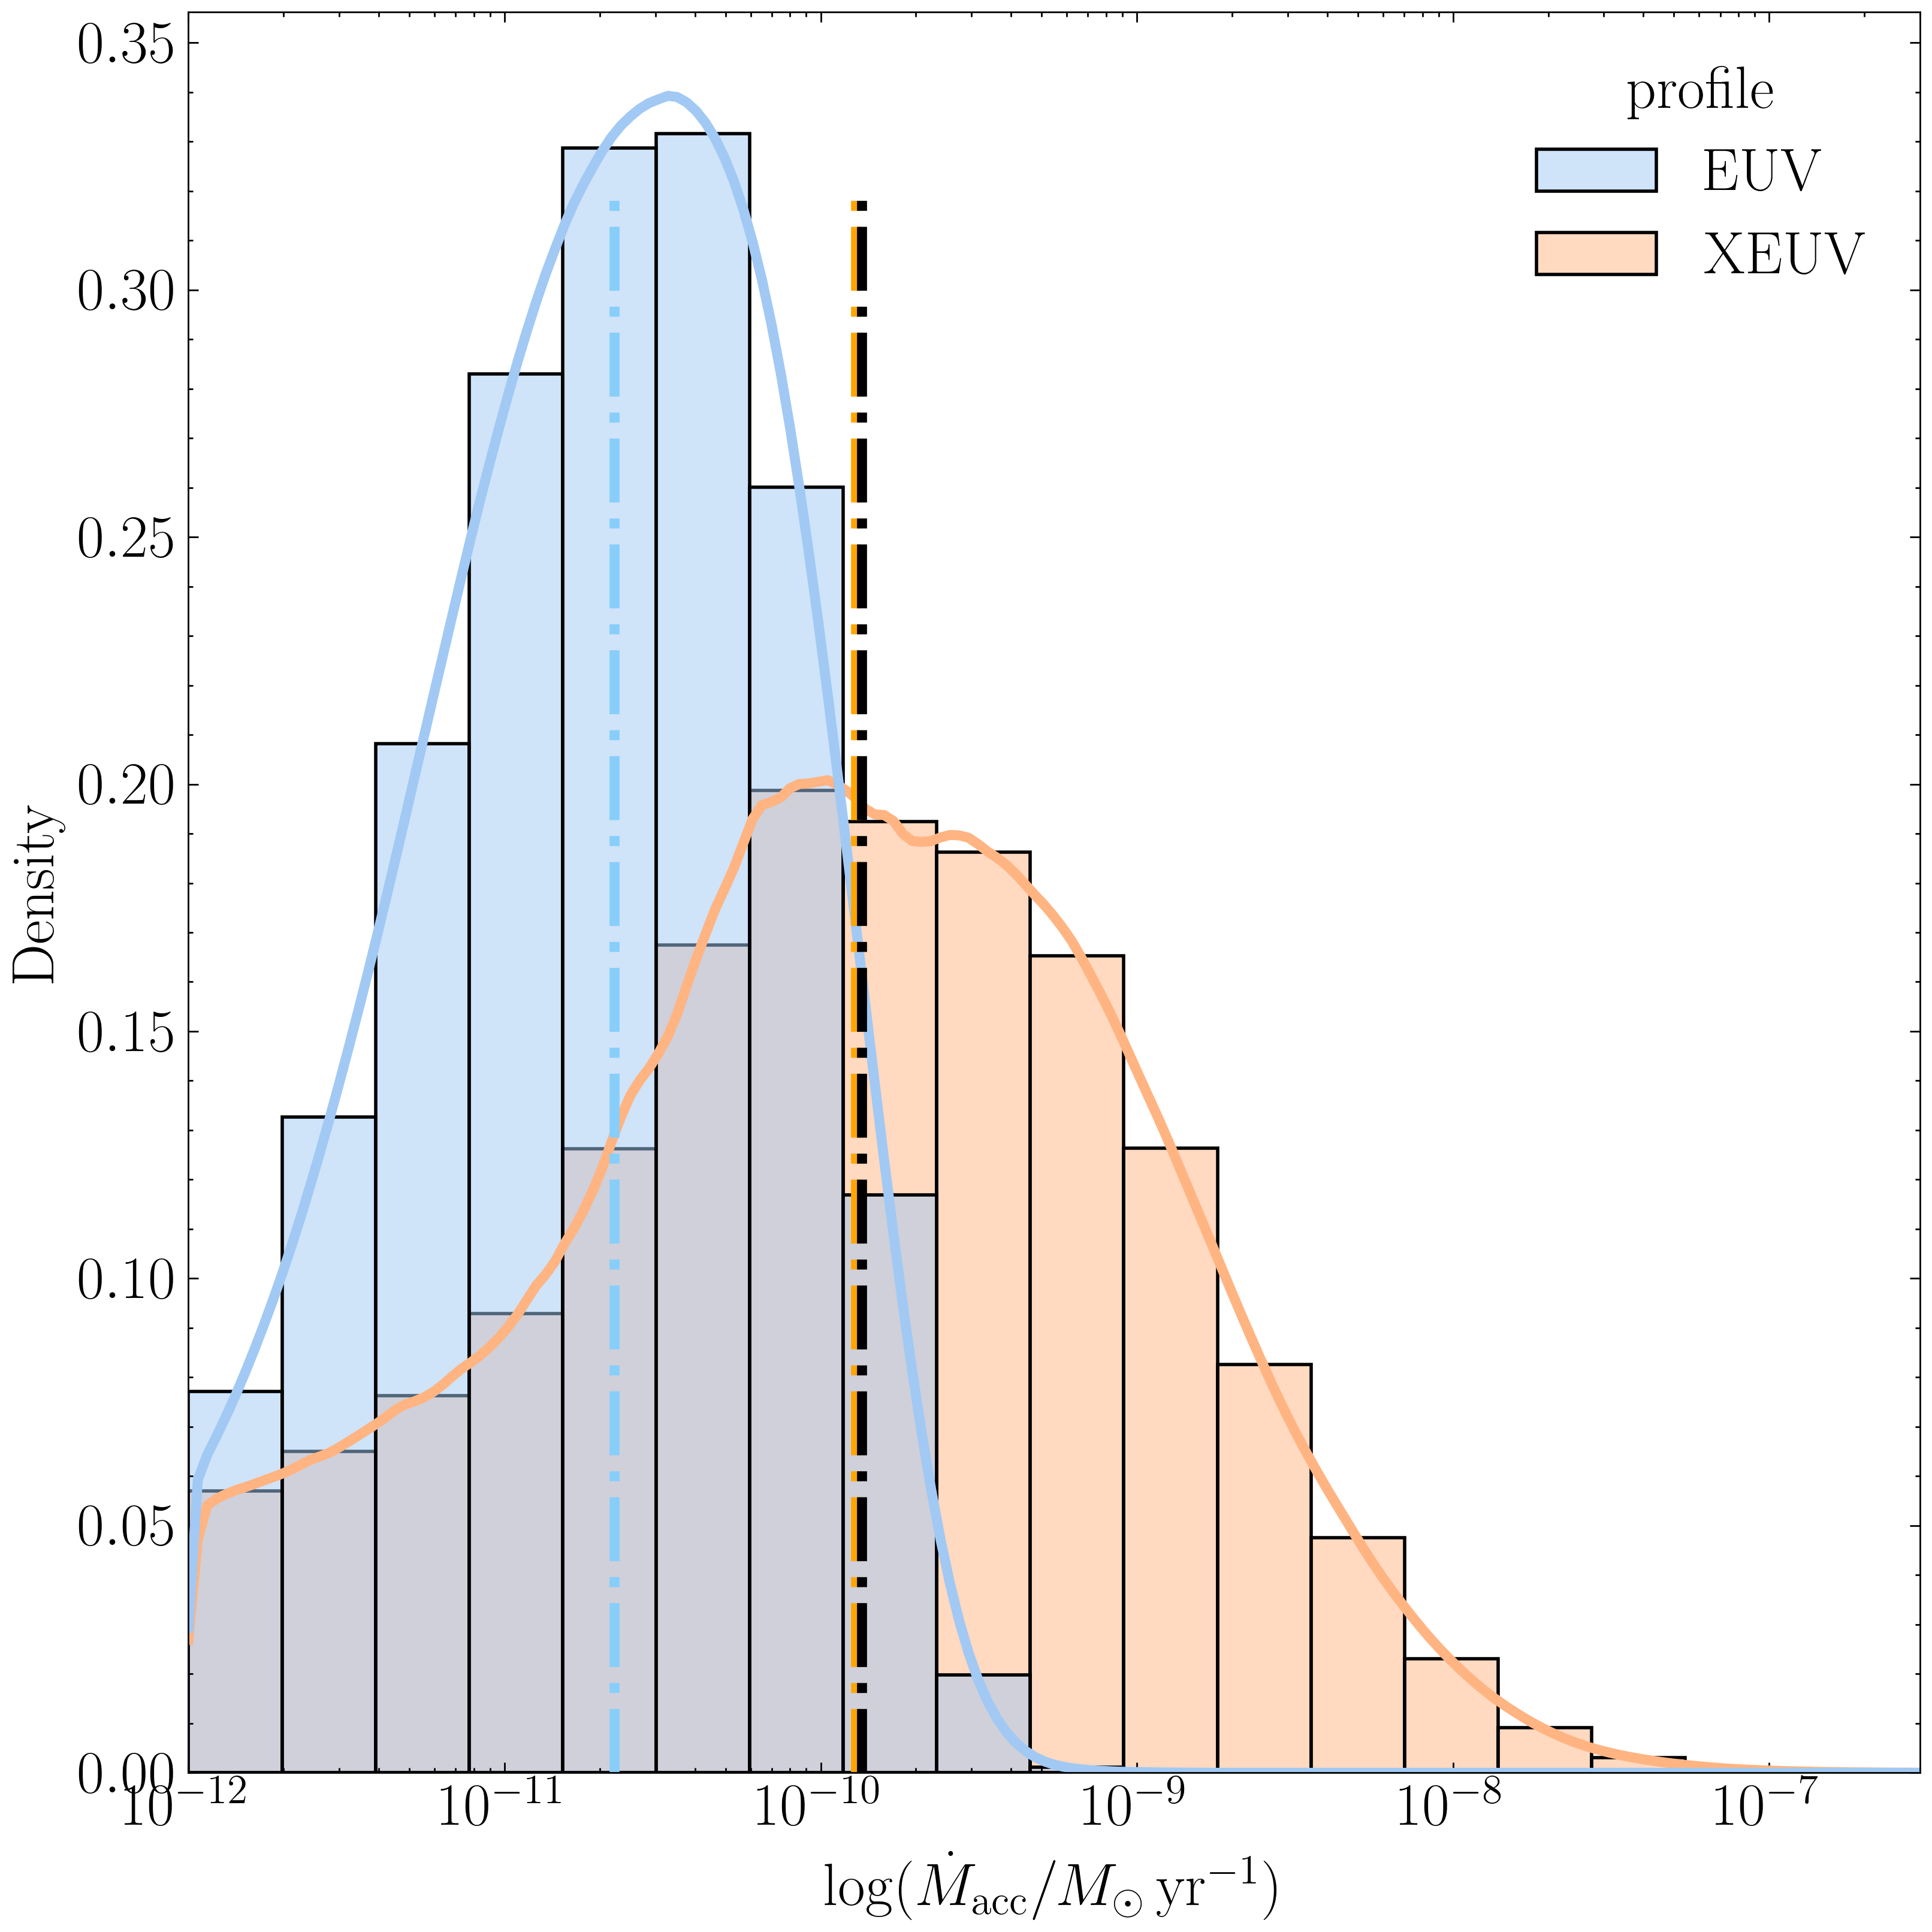
\includegraphics[width=\columnwidth]{Fig7}
    \caption{Histogram of the accretion rate density distribution in the EUV (blue) and XEUV (green) population synthesis. The KDE is overplotted with a blue and green solid line for the EUV and XEUV distributions respectively, and the median values are plotted with dotted-dashed lines. For direct comparison the median accretion rate of the low-accretors population is plotted with a black dotted-dashed line.\label{fig:hist_mdot}}
\end{figure}

We compared finally the distribution of disc fractions as a function of age, calculated as the time at which the accretion rate drops below $10^{-11}$ M$_\odot$ yr$^{-1}$ in our population synthesis with the observed distribution of disc fraction (Figure~\ref{fig:frac_time}, black lines). As expected the EUV distribution fits perfectly, as we choose the parameter space in order to fit it for the median stellar mass and EUV ionizing field. The XEUV distribution is also very accurate in describing the observed star forming region population with the only constraint of an initial disc mass of $0.1$ M$_\star$.

%For the case of X-ray photoevaporation the probability of finding an object at a given accretion rates changes as a function of age of the population. However for objects older than approximately 1~Myr it is clearly not improbable to find objects at rates of order $10^{-10}M_{\odot}/yr$. In particular for objects older than about 5 Myr the probability distribution peaks indeed at these values. For lower accretion rates the probabilty decreases sharply for all ages, indicating that the lowest accretors of a population of discs being dissipated by X-ray photoevaporation is indeed to be found accreting at rates of order $10^{-10} M_{\odot}/yr$ as observed by T22. 
%This can be clearly seen in Figure?? where the probability of an object accreting at a given rate is plotted for a few typical ages. {\color{red} make this figure}. 


%For the case of EUV photoevaporation.... 

\subsection{Mass dependent results}

The results shown in the previous section assume a well-sampled IMF, which implies that objects at the lower end of the mass range are the most abundant (see Figure~\ref{fig:hist} panel a). However the sample of low accretors from \citet{Thanathibodee2023} includes only $24$ objects with masses ranging between $0.1$ and $1.39$ M$_\odot$. The majority of which have masses between $0.5$ and $0.6$ M$_\odot$, resulting in a significant different stellar mass function with respect to the adopted IMF.

In Figure~\ref{fig:frac_time} we divided our sample in three different mass bins in order to understand the effect of stellar mass on the disc lifetime. In the top panel the XEUV profile shows little variation as a function of stellar mass, with a trend of decreasing lifetimes for increasing stellar masses, which is consistent with current observations {\color{red} reference?}. In the bottom panel, the EUV profile shows a stronger dependence on the stellar mass, with an inverse trend of decreasing disc lifetime for smaller mass stars. The overall distribution in this case fits the observational data because of the adopted IMF, but it would overpredict the disc fractions for the stellar mass distribution studied in \citet{Thanathibodee2023}.
%, as shown in Figure~\ref{fig:mstar_comparison}.

%The accretion rate values reported by \citet{Thanathibodee2023} do not show any obvious correlation with the object mass.
%In Figures?? to??? we show the accretion rate probabilities for our populations when we restrict the mass ranges to low (0.1-0.3), intermediate (0.3-0.6), high (0.7-0.9). 
{\color{red} does it add information including Figure 2 for the different stellar mass bins? (maximum of 5 pages getting closer)}.
\begin{figure}
    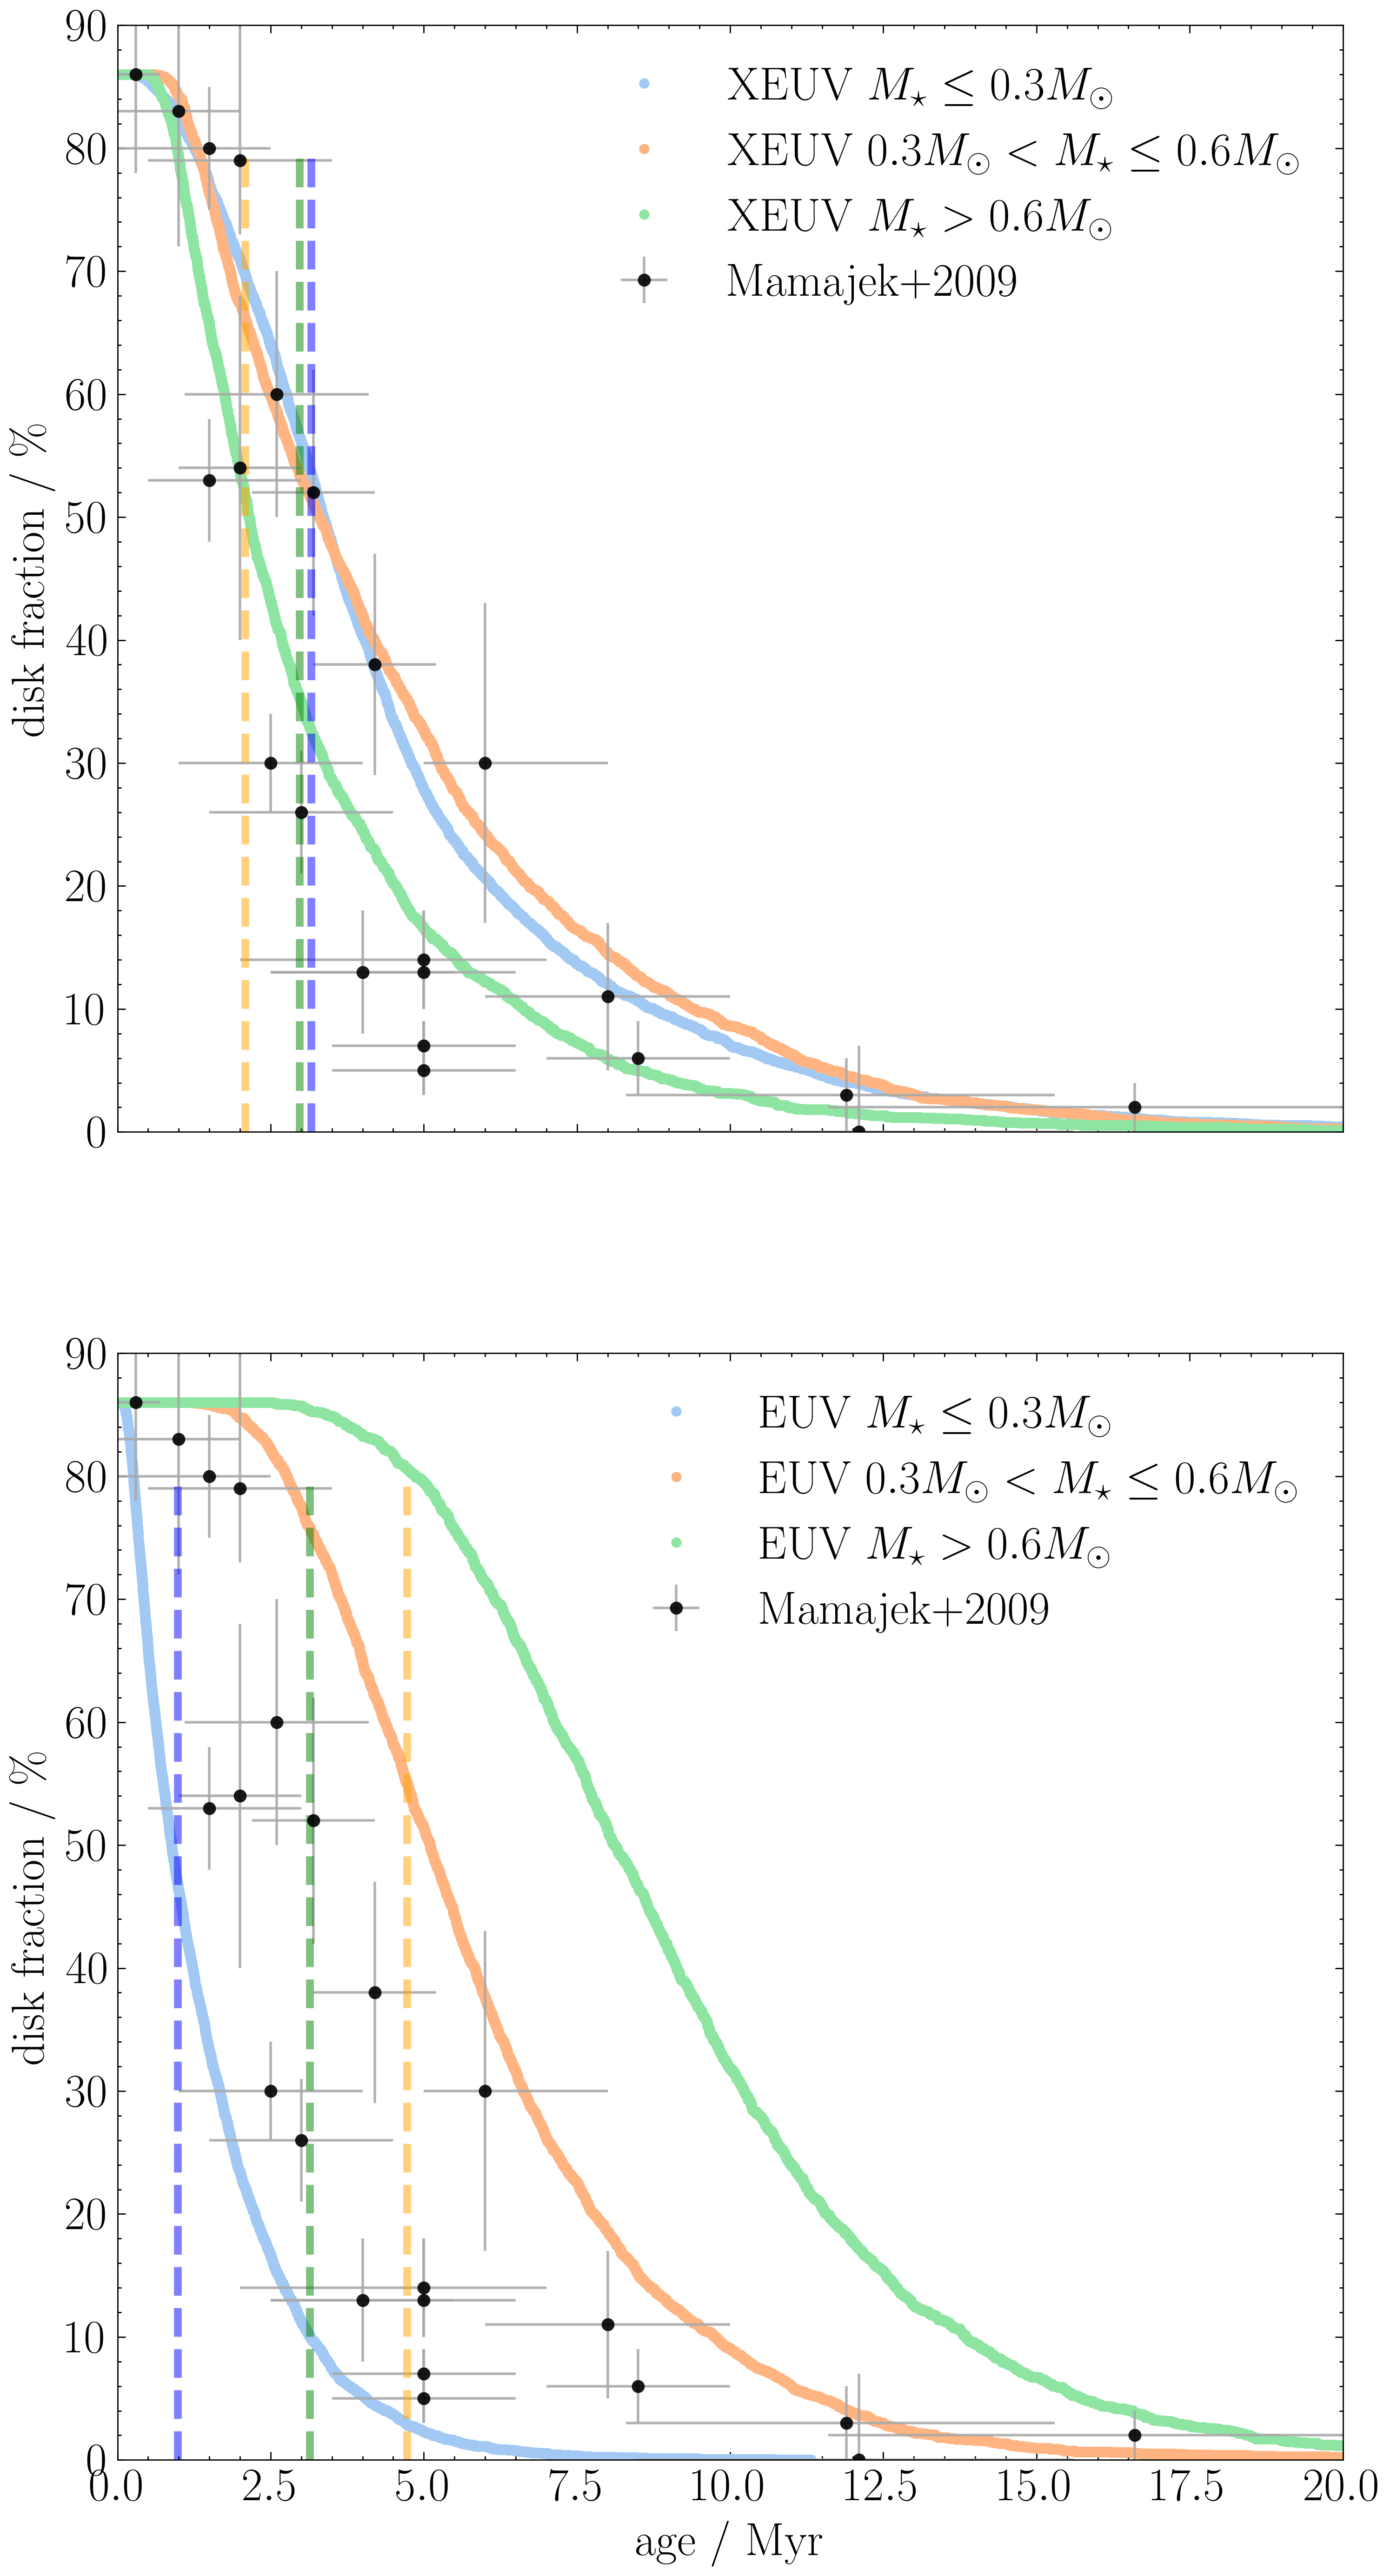
\includegraphics[width=0.92\columnwidth]{Fig8}
    \caption{Disc fraction as a function of disc lifetime for the XEUV (top panel) and EUV (bottom panel) synthetic populations compared with the observational data from \citet{Mamajek2009}, divided in 3 stellar mass bins. The median disc lifetime are plotted with dashed vertical lines. The median disc life-time increases with stellar mass for the EUV models, while it decreases for the XEUV models. \label{fig:frac_time}}
\end{figure}

%\begin{figure}
%    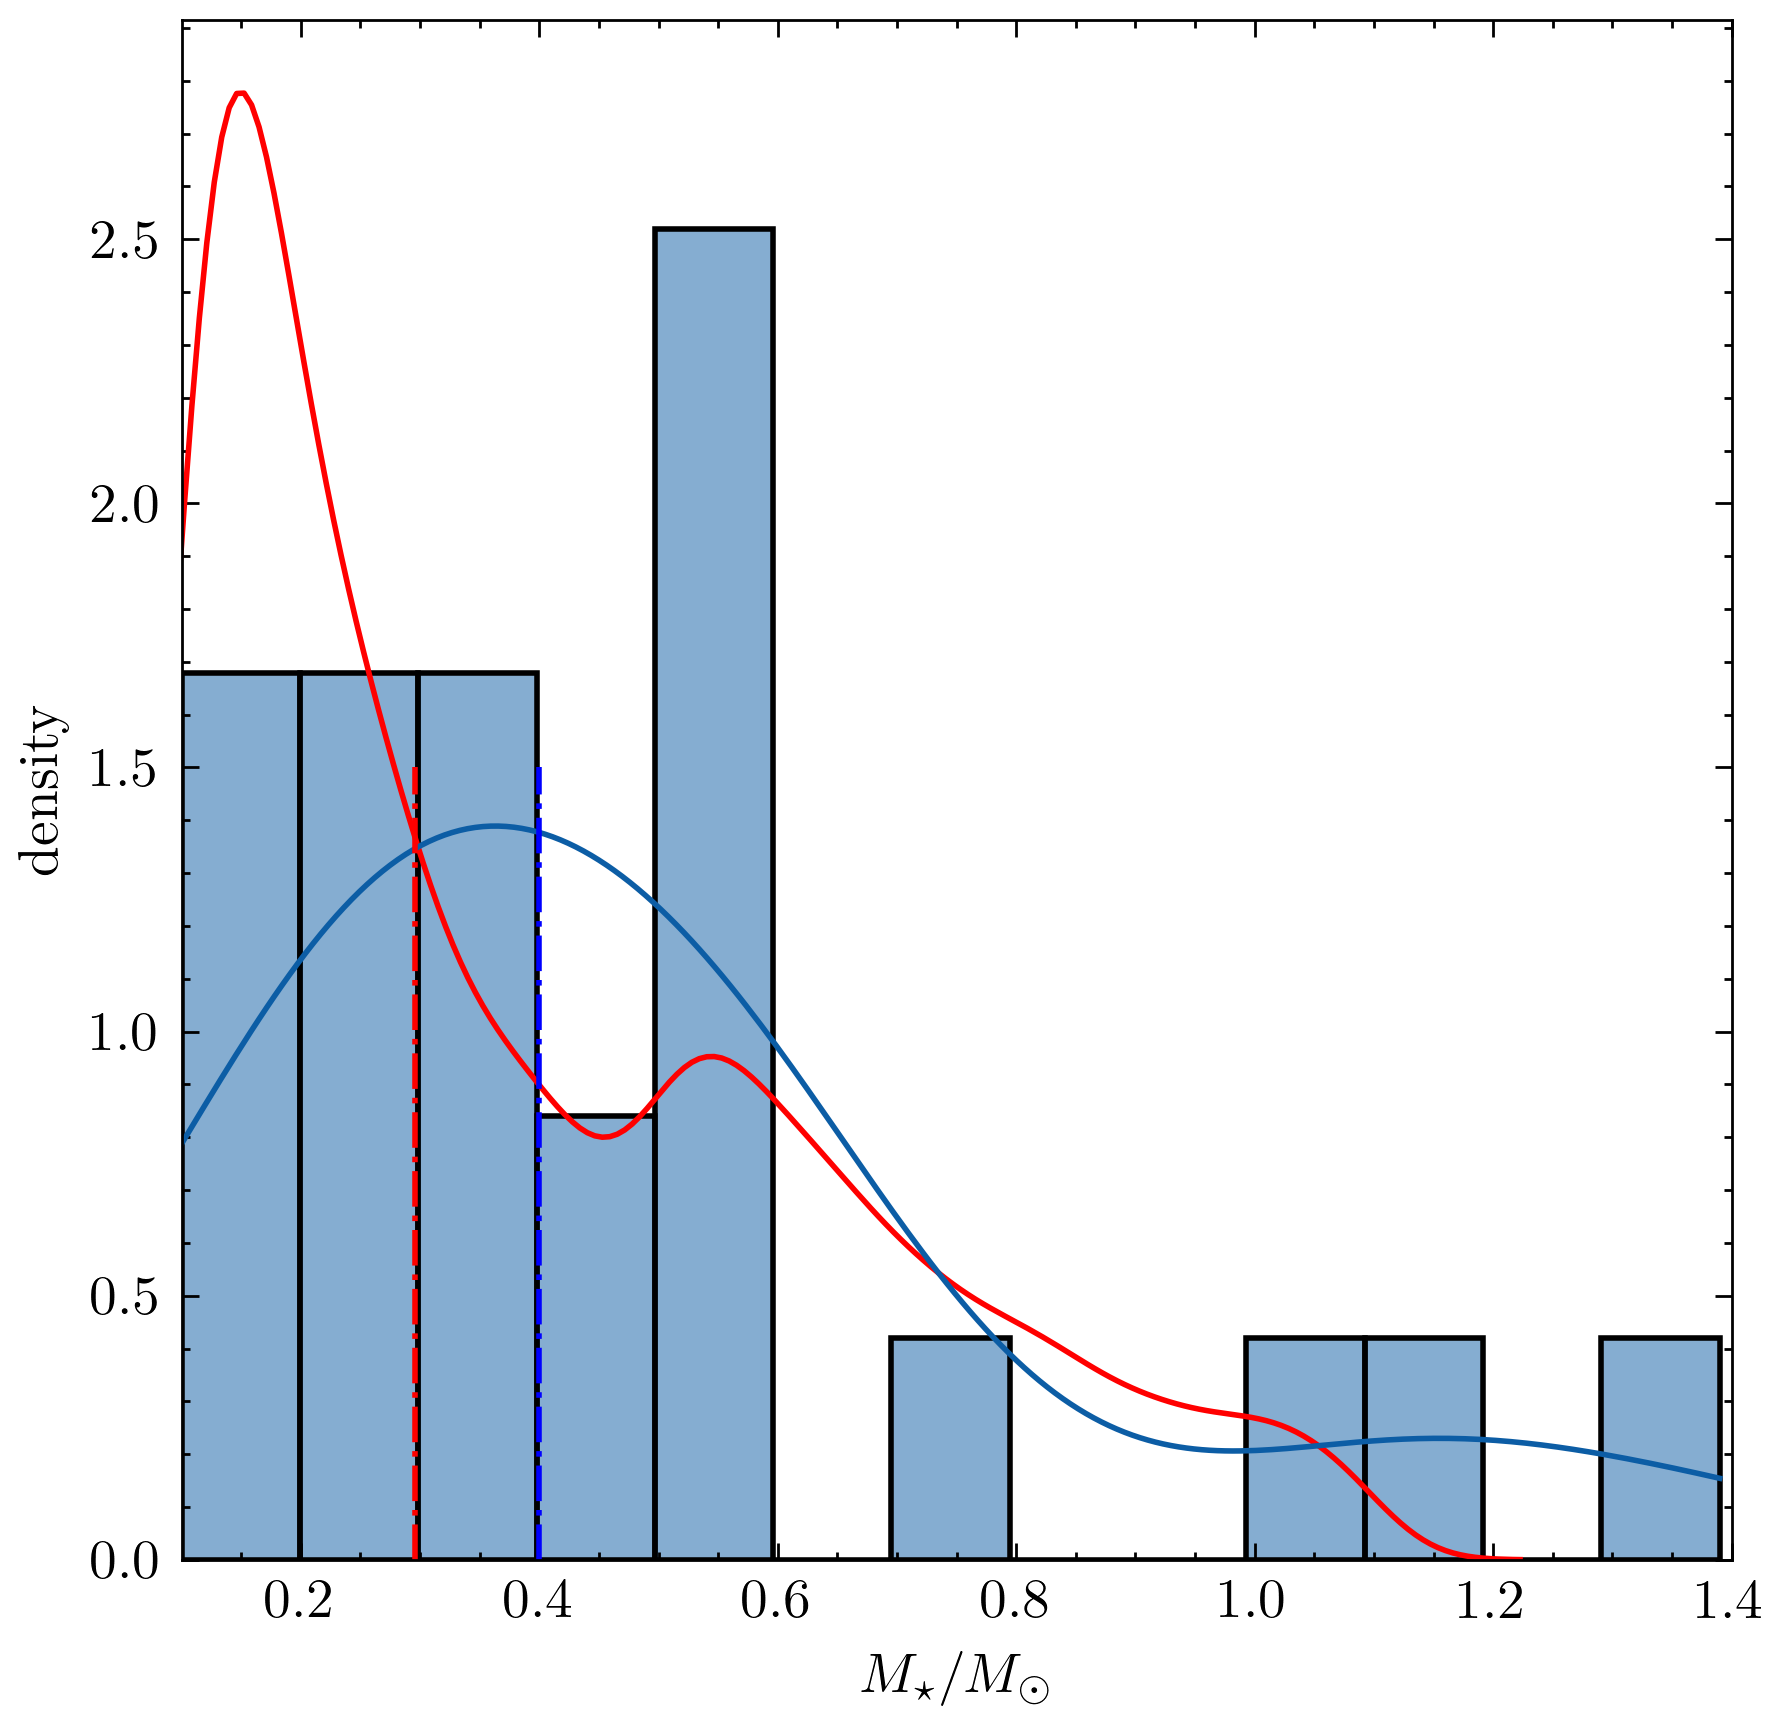
\includegraphics[width=0.92\columnwidth]{Mstar_comparison.png}
%    \caption{Stellar mass distribution of the low-accretor population in \citet{Thanathibodee2023} with overplotted KDE in a solid blue line, compared with the IMF adopted in this work shown with a red solid line. The median values of the two distributions are shown with blue and red dotted-dashed line, respectively.  \label{fig:mstar_comparison}}
%\end{figure}

\subsection{Low-accretors variability}

\citet{Fang2023} obtained the accretion rate of a large sample in Upper Sco adopting high-resolution optical spectra from H$\alpha$ line profiles. Comparing their results with the ones measured for the same star forming region by \citet{Manara2020}, fitting simultaneously the stellar photosphere and Balmer continuous emission, they find a large spread (see their Figure~29) going to more than one order of magnitude, especially for the population of low-accretors. Comparing the low accretors with the ones derived fitting the He I $\lambda10830$ line profiles in \citet{Thanathibodee2023} they found further differences in disc classification and accretion rates. This points towards a general difficulty in classifying low accretors based on line profiles, and their intrinsic variability that should be studied further.

\section{Conclusions}\label{sec:conclusions}

We studied the influence of different internal photoevaporation prescriptions on the physical limit of observed low-accretors. We found that:
\begin{itemize}
  \item internal EUV and X-ray photoevaporation can both explain the observed accretion rates in the low-accretor sample;
  \item the constraints that the EUV internal photoevaporation needs to explain the observed disk lifetime are much more strict than the X-ray driven disc evolution (see eq.~\ref{eq:r1_alpha});
  \item the low-accretors are part of the bulk distribution of X-ray driven photoevaporation (with the median accretion rate overlapping with the one from the sample from \citet{Thanathibodee2023}), while they represent the upper end of the EUV accretors (see Figures~\ref{fig:mdot_age},\ref{fig:hist_mdot});
  \item the dependance of the disk fraction on the stellar mass is stronger for the EUV profiles which is in tension with the observed low accretor population with similar accretion rate across a wide range of stellar masses.
\end{itemize}

\section*{Acknowledgements}

%%%%%%%%%%%%%%%%%%%%%%%%%%%%%%%%%%%%%%%%%%%%%%%%%%
\section*{Data Availability}

The data for the population synthesis calculations is available at \href{https://github.com/GiovanniPicogna/low-accretors}{https://github.com/GiovanniPicogna/low-accretors}

%%%%%%%%%%%%%%%%%%%% REFERENCES %%%%%%%%%%%%%%%%%%

\bibliographystyle{mnras}
\bibliography{lib}

%%%%%%%%%%%%%%%%%%%%%%%%%%%%%%%%%%%%%%%%%%%%%%%%%%

%%%%%%%%%%%%%%%%% APPENDICES %%%%%%%%%%%%%%%%%%%%%

\appendix

%%%%%%%%%%%%%%%%%%%%%%%%%%%%%%%%%%%%%%%%%%%%%%%%%%

% Don't change these lines
\bsp	% typesetting comment
\label{lastpage}
\end{document}

% End of mnras_template.tex
